% =============================================================================
% ADHD Second Brain — FYP Report
% NTU College of Computing and Data Science
% Academic Year 2025/2026
% =============================================================================
\documentclass[12pt,a4paper,oneside]{report}

% ── Page geometry (NTU CCDS template) ────────────────────────────────────────
\usepackage[
  top=30mm,
  bottom=30mm,
  left=35mm,
  right=30mm
]{geometry}

% ── Font: Times New Roman equivalent ────────────────────────────────────────
\usepackage{mathptmx}
\usepackage[T1]{fontenc}
\usepackage[utf8]{inputenc}

% ── Spacing ──────────────────────────────────────────────────────────────────
\usepackage{setspace}
\onehalfspacing

% ── Graphics and figures ─────────────────────────────────────────────────────
\usepackage{graphicx}
\graphicspath{{figures/}}
\usepackage{caption}
\captionsetup{font=small}
\usepackage{subcaption}

% ── Tables ───────────────────────────────────────────────────────────────────
\usepackage{booktabs}
\usepackage{array}
\usepackage{tabularx}
\usepackage{longtable}
\usepackage{multirow}

% ── Mathematics and symbols ──────────────────────────────────────────────────
\usepackage{amsmath}
\usepackage{amssymb}
\usepackage{pifont}

\newcommand{\cmark}{\ding{51}}
\newcommand{\xmark}{\ding{55}}

% ── Colours and code listings ────────────────────────────────────────────────
\usepackage{xcolor}
\usepackage{listings}
\lstset{
  basicstyle=\ttfamily\small,
  breaklines=true,
  frame=single,
  numbers=left,
  numberstyle=\tiny\color{gray},
  keywordstyle=\color{blue},
  commentstyle=\color{green!50!black},
  stringstyle=\color{red!60!black},
  tabsize=4,
  showstringspaces=false
}

% ── Drawing ──────────────────────────────────────────────────────────────────
\usepackage{tikz}
\usepackage{pgfplots}
\pgfplotsset{compat=1.18}
\usetikzlibrary{arrows.meta,positioning,shapes.geometric,calc,fit,backgrounds,decorations.pathreplacing}

% ── Bibliography ─────────────────────────────────────────────────────────────
\usepackage[
  backend=biber,
  style=numeric,
  sorting=none,
  maxbibnames=99
]{biblatex}
\addbibresource{references.bib}

% ── Hyperlinks and cross-references ──────────────────────────────────────────
\usepackage{hyperref}
\hypersetup{
  colorlinks=true,
  linkcolor=black,
  citecolor=blue!60!black,
  urlcolor=blue!70!black,
  bookmarksnumbered=true,
  pdfstartview={FitH}
}
\usepackage{cleveref}

% ── Miscellaneous ────────────────────────────────────────────────────────────
\usepackage{enumitem}
\usepackage{url}
\usepackage{float}
\usepackage{microtype}
\usepackage{parskip}

% ── Chapter heading style ────────────────────────────────────────────────────
\usepackage{titlesec}
\titleformat{\chapter}[display]
  {\normalfont\huge\bfseries}
  {\chaptertitlename\ \thechapter}{20pt}{\Huge}
\titlespacing*{\chapter}{0pt}{-20pt}{20pt}

% =============================================================================
% DOCUMENT
% =============================================================================
\begin{document}

% ── Front matter (roman numerals) ────────────────────────────────────────────
\pagenumbering{roman}
% =============================================================================
% Front Matter
% =============================================================================

% ── Title Page ───────────────────────────────────────────────────────────────
\begin{titlepage}
  \centering
  \vspace*{0.5cm}

  
\includegraphics[width=0.55\textwidth]{ntu-logo.png}

  \vspace{2.5cm}

  {\LARGE\bfseries
    ADHD Second Brain:\\[8pt]
    An On-Device AI-Powered macOS Application\\[8pt]
    for ADHD Productivity and Digital Wellbeing
  }

  \vspace{2.5cm}

  {\large
    Avdhesh Shrikant Charjan\\[4pt]
    U2123954A
  }

  \vspace{1.5cm}

  {\normalsize
    Project Supervisor: Prof Erik Cambria, Dr Rui Mao\\[6pt]
    Examiner: Assoc Prof Stefano Vittorino Albrecht
  }

  \vspace{2cm}

  {\large
    College of Computing and Data Science\\[4pt]
    Academic Year 2025/2026
  }

  \vfill
\end{titlepage}

% ── Statement of Originality ─────────────────────────────────────────────────
\chapter*{Statement of Originality}
\addcontentsline{toc}{chapter}{Statement of Originality}

I hereby certify that the work embodied in this report is the result of original research and has not been submitted for a higher degree to any other University or Institution.

\vspace{1cm}

\noindent\textbf{Disclosure of AI Tool Usage}

\noindent In accordance with NTU's policy on the use of generative AI tools in academic work (effective November 2025), the following AI tools were used during the preparation of this report:

\begin{itemize}[leftmargin=2cm]
  \item \textbf{Claude (Anthropic)}: code review and literature synthesis.
  \item \textbf{ChatGPT (OpenAI)}: brainstorming and proofreading selected sections.
\end{itemize}

\noindent All AI-generated content was reviewed, verified, and substantially revised by the author. The intellectual contributions, system design, implementation, and evaluation are entirely the author's own work.

\vspace{2cm}

\begin{tabular}{@{}ll}
  \rule{6cm}{0.4pt} & \rule{4cm}{0.4pt} \\
  Signature                & Date
\end{tabular}

\newpage

% ── Supervisor Declaration Statement ─────────────────────────────────────────
\chapter*{Supervisor Declaration Statement}
\addcontentsline{toc}{chapter}{Supervisor Declaration Statement}

I have reviewed the content and presentation of this report and confirm that it represents the student's own work, conducted under my supervision.

\vspace{3cm}

\begin{tabular}{@{}ll}
  \rule{6cm}{0.4pt} & \rule{4cm}{0.4pt} \\
  Supervisor Signature     & Date
\end{tabular}

\newpage

% ── Authorship Attribution Statement ─────────────────────────────────────────
\chapter*{Authorship Attribution Statement}
\addcontentsline{toc}{chapter}{Authorship Attribution Statement}

This report is written entirely by the undersigned. All work presented in this report was carried out by the author unless otherwise stated. Where the work of others has been used, it has been duly acknowledged and referenced.

The following contributions are noted:

\begin{itemize}[leftmargin=2cm]
  \item The SenticNet APIs (Chapter~4, Section~4.4) were provided by the SenticNet research group at NTU.
  \item The Mem0 memory framework (Chapter~4, Section~4.5) is an open-source library used under the Apache~2.0 licence.
  \item The Apple MLX framework (Chapter~4, Section~4.2) is an open-source library developed by Apple Inc.
\end{itemize}

\vspace{2cm}

\begin{tabular}{@{}ll}
  \rule{6cm}{0.4pt} & \rule{4cm}{0.4pt} \\
  Signature                & Date
\end{tabular}

\newpage

% ── Abstract ─────────────────────────────────────────────────────────────────
\chapter*{Abstract}
\addcontentsline{toc}{chapter}{Abstract}

Attention-Deficit/Hyperactivity Disorder (ADHD) affects an estimated 2.58\% to 6.76\% of the global adult population, imposing a substantial economic burden of approximately USD~4,336 per affected worker per year in lost productivity. The proliferation of digital devices and persistent connectivity has compounded core ADHD symptoms, including attentional dysregulation, working memory deficits, and impaired executive function. Despite the prevalence of productivity applications on the market, no integrated desktop tool existed that combined conversational coaching, real-time emotion awareness, screen activity monitoring, and persistent semantic memory within a single privacy-preserving framework.

This project developed an on-device AI-powered macOS application that addressed these gaps through the integration of several complementary subsystems. A Qwen3-4B large language model, executed locally via the Apple MLX framework, provided conversational coaching at 37.1 tokens per second. A SetFit contrastive learning pipeline achieved 86\% emotion classification accuracy across six ADHD-specific affective categories using only 210 training sentences. SenticNet affective computing, accessed through 13 application programming interfaces and grounded in the Hourglass of Emotions model, supplied fine-grained sentiment and sentic features with 100\% reliability. Mem0 semantic memory, backed by pgvector, attained 95\% top-1 relevance in context retrieval. A five-tier activity classification engine processed screen titles at 549 titles per second, and Just-in-Time Adaptive Interventions, structured around Barkley's executive function domains, delivered context-sensitive behavioural nudges.

Evaluation demonstrated that the system consumed 21,314 millijoules per inference, representing approximately 1.4\% battery drain per hour, while maintaining a peak memory footprint below 3 gigabytes. All predefined project objectives were exceeded. The application constituted the first macOS-native ADHD assistant with a fully on-device large language model, addressed eight identified market gaps, and contributed an open-source evaluation framework with reproducible benchmarks.

\newpage

% ── Acknowledgements ─────────────────────────────────────────────────────────
\chapter*{Acknowledgements}
\addcontentsline{toc}{chapter}{Acknowledgements}

% TODO: Replace with actual acknowledgements.
I would like to express my sincere gratitude to my supervisor for the guidance and support throughout this project. I also thank the SenticNet research group at NTU for providing access to the SenticNet APIs. Finally, I am grateful to my family and friends for their encouragement and patience.

\newpage

% ── Table of Contents ────────────────────────────────────────────────────────
\tableofcontents
\newpage

% ── List of Figures ──────────────────────────────────────────────────────────
\listoffigures
\addcontentsline{toc}{chapter}{List of Figures}
\newpage

% ── List of Tables ───────────────────────────────────────────────────────────
\listoftables
\addcontentsline{toc}{chapter}{List of Tables}
\newpage

% ── List of Abbreviations ────────────────────────────────────────────────────
\chapter*{List of Abbreviations}
\addcontentsline{toc}{chapter}{List of Abbreviations}

\begin{longtable}{@{}l l@{}}
  \toprule
  \textbf{Abbreviation} & \textbf{Definition} \\
  \midrule
  \endfirsthead
  \toprule
  \textbf{Abbreviation} & \textbf{Definition} \\
  \midrule
  \endhead
  \bottomrule
  \endfoot
  ADHD   & Attention-Deficit/Hyperactivity Disorder \\
  AI     & Artificial Intelligence \\
  ANE    & Apple Neural Engine \\
  API    & Application Programming Interface \\
  ASRS   & Adult ADHD Self-Report Scale \\
  CBM    & Concept Bottleneck Model \\
  CBT    & Cognitive Behavioural Therapy \\
  CLI    & Command-Line Interface \\
  CPU    & Central Processing Unit \\
  CV     & Coefficient of Variation \\
  DRAM   & Dynamic Random-Access Memory \\
  E2E    & End-to-End \\
  EF     & Executive Function \\
  F1     & F1-Score (harmonic mean of precision and recall) \\
  GPU    & Graphics Processing Unit \\
  HRV    & Heart Rate Variability \\
  IEEE   & Institute of Electrical and Electronics Engineers \\
  IRB    & Institutional Review Board \\
  JITAI  & Just-in-Time Adaptive Intervention \\
  LLM    & Large Language Model \\
  LoRA   & Low-Rank Adaptation \\
  MLX    & Apple Machine Learning Framework \\
  MPS    & Metal Performance Shaders \\
  NLP    & Natural Language Processing \\
  NTU    & Nanyang Technological University \\
  PARA   & Projects, Areas, Resources, Archives \\
  PKM    & Personal Knowledge Management \\
  QLoRA  & Quantised Low-Rank Adaptation \\
  RAG    & Retrieval-Augmented Generation \\
  RSS    & Resident Set Size \\
  STS    & Semantic Textual Similarity \\
  SUS    & System Usability Scale \\
  XAI    & Explainable Artificial Intelligence \\
\end{longtable}


% ── Main chapters (arabic numerals) ──────────────────────────────────────────
\pagenumbering{arabic}
% =============================================================================
% Chapter 1 — Introduction
% =============================================================================
\chapter{Introduction}
\label{ch:introduction}

Attention-Deficit/Hyperactivity Disorder (ADHD) is among the most prevalent neurodevelopmental conditions worldwide, yet digital interventions for adults with ADHD remain remarkably underdeveloped. This chapter motivates the need for an integrated, privacy-preserving desktop application that combines on-device language modelling, affective computing, screen activity monitoring, and persistent memory to support adults with ADHD in knowledge work. The chapter articulates the specific problem, defines measurable objectives, delineates scope and limitations, and summarises the contributions of this work.

% -----------------------------------------------------------------------------
\section{Background and Motivation}
\label{sec:background}

\subsection{ADHD Prevalence and the Executive Function Deficit}
\label{subsec:adhd-prevalence}

Attention-Deficit/Hyperactivity Disorder is a neurodevelopmental condition characterised not merely by difficulties sustaining attention, but by pervasive impairments in executive function---the set of cognitive processes that enable goal-directed behaviour, working memory, inhibitory control, and cognitive flexibility \cite{diamond2013}. Meta-analytic estimates place the global adult prevalence of ADHD between 2.58\% and 6.76\% \cite{faraone2021, song2021}, translating to over 200 million adults worldwide who navigate daily life with executive function profiles that diverge substantially from the neurotypical baseline upon which most productivity tools and digital interfaces are designed. ADHD in adults is associated with reduced occupational attainment, higher rates of job turnover, and elevated risk of comorbid anxiety and mood disorders, yet the technology ecosystem has been slow to develop tools that accommodate this specific cognitive profile.

\subsection{Economic Impact and the Knowledge Worker Gap}
\label{subsec:economic-impact}

The economic burden of adult ADHD is substantial. Barkley and Murphy estimated the excess annual cost at \$4,336 per worker per year, attributable to reduced productivity, increased absenteeism, and elevated error rates \cite{barkley2010}. In the knowledge economy, where the desktop computer is the primary instrument of production, this cost accrues overwhelmingly at the human-computer interface. Adults with ADHD spend most of their working hours interacting with desktop applications---email clients, web browsers, code editors---yet these applications assume intact working memory, sustained attention, and consistent self-regulation. An application that could reduce even a fraction of this productivity loss would need to understand what the user is doing, how the user is feeling, and what the user has done before, all without sending sensitive data to external servers.

\subsection{The Digital Distraction Paradox}
\label{subsec:digital-distraction}

A particularly vexing challenge is the digital distraction paradox: ADHD predisposes individuals to distraction by digital stimuli, while excessive digital engagement exacerbates attentional difficulties \cite{thorell2022, dontre2021}. The desktop computer is simultaneously the primary workspace and the primary distraction vector. Existing approaches---website blockers, application timers, focus modes---treat the symptom rather than the cause, imposing external constraints without understanding the cognitive or affective state that precipitated the distraction. Despite growing interest in digital mental health interventions, the evidence base for ADHD-specific applications remains thin, with a recent meta-analysis finding only a modest effect size of Hedges' $g = -0.32$ \cite{garciaperal2025}. Among ADHD-specific tools, Brain.fm is one of the very few with peer-reviewed evidence \cite{woods2024}; the broader landscape consists overwhelmingly of static task managers and timers that lack adaptive intelligence, affective awareness, or personalised coaching. A more effective intervention would monitor screen activity in real time, detect drift from productive work, and intervene with context-aware coaching that accounts for the user's emotional state and historical patterns.

\subsection{Emotion Dysregulation as a Core Symptom}
\label{subsec:emotion-dysregulation}

Recent clinical research has increasingly recognised emotion dysregulation not as a mere comorbidity, but as a fourth core symptom of ADHD alongside inattention, hyperactivity, and impulsivity \cite{beattie2025}. Adults with ADHD frequently experience rapid, intense emotional responses---frustration when tasks prove difficult, anxiety when deadlines loom, and overwhelming cognitive overload when demands exceed executive capacity. These affective states are primary drivers of task abandonment, not incidental to it. Any comprehensive support system must therefore incorporate affective awareness: an application that detects frustration or anxiety and responds with appropriately timed, empathetic coaching has the potential to interrupt the emotion--distraction--guilt cycle that characterises much of the ADHD experience in knowledge work.

\subsection{The Second Brain Paradigm and the Privacy Imperative}
\label{subsec:second-brain-privacy}

The ``Second Brain'' paradigm, popularised by Forte \cite{forte2022}, advocates for the systematic externalisation of knowledge into a persistent digital system that augments human memory. This paradigm is especially relevant for adults with ADHD, whose working memory deficits mean that valuable insights and contextual knowledge are routinely lost between sessions. However, the tools most commonly associated with this paradigm---Notion, Obsidian, Roam Research---require precisely the executive functions that ADHD impairs: consistent categorisation, regular review, and disciplined capture habits. A truly ADHD-appropriate Second Brain must automate the capture and organisation process, requiring minimal executive overhead from the user.

Such a system produces data of extraordinary sensitivity---screen content, emotional states, conversational transcripts---creating unacceptable privacy risks if transmitted to cloud servers. Recent advances in edge AI have made on-device processing a viable alternative. The MLX framework, developed by Apple Machine Learning Research, enables efficient neural network inference on Apple Silicon hardware \cite{hannun2023}, and models such as Qwen3-4B \cite{yang2025} achieve competitive performance while fitting within the memory constraints of consumer hardware. Together, these technologies make it feasible to run a capable language model, an emotion classifier, and a memory system entirely on the user's device.

% -----------------------------------------------------------------------------
\section{Problem Statement}
\label{sec:problem-statement}

Adults with ADHD who work primarily on desktop computers face a fragmented landscape of support tools, typically requiring three to five separate applications: a task manager, a focus timer, a note-taking system, a calendar, and possibly a mood tracker. Each operates in isolation, unaware of the user's activity in other applications, emotional state, or historical patterns. This fragmentation is itself an ADHD tax---the cognitive overhead of switching between tools actively undermines the executive functions the tools are ostensibly designed to support.

From a technical standpoint, no existing application integrates on-device large language model coaching, real-time affective computing, continuous screen activity monitoring, and persistent conversational memory within a single desktop application. Cloud-based solutions exist for individual components but introduce latency, require network connectivity, and create the privacy vulnerabilities discussed in \cref{subsec:second-brain-privacy}. The technical challenge is to unify these capabilities into a coherent, responsive, and private desktop application that runs entirely on consumer hardware.

% -----------------------------------------------------------------------------
\section{Project Objectives}
\label{sec:objectives}

This project aims to design, implement, and evaluate a desktop application---the ADHD Second Brain---that provides integrated, privacy-preserving cognitive support for adults with ADHD. The application targets macOS on Apple Silicon hardware, leveraging the MLX framework for on-device inference. Five specific, measurable objectives guide the project.

\textbf{Objective 1: On-Device LLM Coaching.} The application shall provide real-time conversational coaching through Qwen3-4B on the MLX framework, targeting at least 30 tokens per second. The achieved throughput of 37.1 tok/s exceeds the target by 23.7\%.

\textbf{Objective 2: Emotion Classification.} The application shall classify user-expressed emotion into six ADHD-relevant categories with at least 80\% accuracy. The achieved accuracy of 86\% (macro-F1 0.862), trained on only 210 sentences, demonstrates that few-shot contrastive learning yields clinically useful classifiers.

\textbf{Objective 3: Screen Activity Classification.} The application shall classify active window titles in real time. The achieved throughput of 549 titles per second, with 78\% resolved by deterministic rules, ensures negligible computational overhead.

\textbf{Objective 4: Persistent Conversational Memory.} The application shall maintain persistent memory using the Mem0 framework, targeting at least 90\% top-1 relevance. The achieved 95\% top-1 hit rate ensures contextually grounded coaching responses.

\textbf{Objective 5: Privacy-Preserving, Energy-Efficient Architecture.} All sensitive data shall be processed on-device. The achieved energy consumption of approximately 1.4\% battery per hour and peak AI memory below 2.5 GB confirm suitability for sustained daily use.

\Cref{tab:objectives-summary} summarises the quantitative targets and achieved results for each objective.

\begin{table}[htbp]
  \centering
  \caption{Summary of project objectives, targets, and achieved results.}
  \label{tab:objectives-summary}
  \begin{tabular}{@{}lll@{}}
    \toprule
    \textbf{Objective}          & \textbf{Target}         & \textbf{Achieved}      \\
    \midrule
    LLM throughput              & $\geq$30 tok/s          & 37.1 tok/s             \\
    Emotion accuracy            & $\geq$80\%              & 86\%                   \\
    Screen classification       & Real-time               & 549 titles/s           \\
    Memory relevance            & $\geq$90\% top-1        & 95\% top-1             \\
    Energy consumption          & $<$2\% battery/hr       & $\sim$1.4\% battery/hr \\
    Peak AI memory              & $<$3 GB                 & $<$2.5 GB              \\
    \bottomrule
  \end{tabular}
\end{table}

% -----------------------------------------------------------------------------
\section{Project Scope and Limitations}
\label{sec:scope}

The scope of this project encompasses the design, implementation, and evaluation of a single-user macOS desktop application targeting Apple Silicon M-series processors. The application is implemented in Python with a Swift-based menu bar interface and comprises five core modules: an on-device LLM coaching engine, an emotion classification pipeline, a screen activity monitor and classifier, a persistent memory system, and a just-in-time adaptive intervention (JITAI) orchestrator. The implementation is accompanied by a comprehensive test suite of over 200 unit, integration, and end-to-end tests. All natural language processing is conducted in English, and the system is designed for individual rather than collaborative use.

Several deliberate limitations bound the project. First, the application targets macOS exclusively, as the MLX framework and Apple Silicon GPU acceleration are platform-specific. Second, emotion detection relies solely on text-based classification of user chat messages; multimodal signals are not incorporated. Third, the project does not include an IRB-approved clinical trial with ADHD-diagnosed participants; evaluation is conducted through automated benchmarks and system-level performance metrics. Fourth, the on-device LLM uses prompt engineering rather than parameter-efficient fine-tuning. Fifth, the emotion classifier is trained on expert-labelled synthetic data rather than clinical data collected from individuals with diagnosed ADHD.

% -----------------------------------------------------------------------------
\section{Contributions and Significance}
\label{sec:contributions}

The primary contribution of this project is the design and implementation of the first integrated desktop application that combines on-device large language model coaching, real-time affective computing, continuous screen activity monitoring, and persistent conversational memory for adults with ADHD. While individual components exist as separate tools or cloud services, no prior work has unified these capabilities into a single, privacy-preserving desktop application optimised for the ADHD cognitive profile. This integration is a clinical necessity, as the fragmentation of support tools imposes precisely the executive overhead that adults with ADHD can least afford.

The project makes four specific technical contributions. First, a four-tier SenticNet integration pipeline that combines API-based affective knowledge with local caching to enrich coaching responses with validated emotional context. Second, a few-shot emotion classification system achieving 86\% accuracy across six ADHD-relevant categories using only 210 labelled sentences, demonstrating that contrastive learning with sentence transformers \cite{reimers2019} can yield clinically useful classifiers without large-scale annotation. Third, a hybrid screen activity classification system processing 549 titles per second, resolving 78\% through deterministic rules and falling back to a 14-class ML classifier with 96.5\% accuracy. Fourth, a persistent memory system achieving 95\% top-1 retrieval relevance. A systematic analysis of nine existing ADHD and productivity applications identifies eight distinct capability gaps that the ADHD Second Brain addresses, positioning it as a fundamentally different category of application.

The broader significance lies in demonstrating that edge AI is viable for mental health applications. By running a 4-billion-parameter language model, an emotion classifier, and a memory system on a consumer laptop with less than 2.5 GB peak AI memory and approximately 1.4\% battery drain per hour, the project establishes that privacy-preserving, always-on cognitive support is technically feasible on current hardware, providing a reference point for any application seeking to deploy sensitive AI capabilities on-device.

% -----------------------------------------------------------------------------
\section{Report Organisation}
\label{sec:report-organisation}

The remainder of this report is organised as follows. \Cref{ch:litrev} reviews the relevant literature on ADHD, digital interventions, affective computing, on-device language models, and memory-augmented AI systems, establishing the theoretical and technical foundations for the system design. \Cref{ch:system_design} presents the system architecture, detailing the design of each module and the rationale for key architectural decisions. \Cref{ch:implementation} describes the implementation of each component, including the emotion classification pipeline, the LLM integration, the screen monitoring system, and the memory framework. \Cref{ch:testing-evaluation} reports the testing methodology and evaluation results, covering unit and integration testing, benchmark performance, and comparative analysis against project objectives. \Cref{ch:conclusion} concludes the report with a summary of achievements, a discussion of limitations, directions for future work, and lessons learned during development.

\input{chapter2-literature-review}
% =============================================================================
% Chapter 3: System Design and Architecture
% =============================================================================
\chapter{System Design and Architecture}
\label{ch:system_design}

This chapter presents the design and architecture of the ADHD Second Brain, an on-device assistant combining affective computing, local large language model inference, and just-in-time adaptive interventions for individuals with ADHD. The system is designed around three principles: (1) privacy-first on-device processing, (2) real-time responsiveness, and (3) interpretable emotional intelligence grounded in established psychological frameworks.

% =============================================================================
\section{Overall System Architecture}
\label{sec:overall_architecture}
% =============================================================================

The system adopts a three-layer architecture comprising a User Layer, a Backend Layer, and a Data Layer. All three layers execute locally, with external calls made only when strictly necessary and never for sensitive screen-capture data. \Cref{fig:system_architecture} provides a high-level overview.

% --- MERMAID BACKUP ---
% flowchart TB
%   subgraph User["User Layer"]
%     A[SwiftUI Menu Bar<br>~25MB RAM]
%     B[React Dashboard<br>Vite]
%     C[OpenClaw<br>Telegram/WhatsApp]
%   end
%   subgraph Backend["Backend Layer - FastAPI :8420"]
%     D[SenticNet Pipeline]
%     E[JITAI Engine]
%     F[MLX Inference<br>Qwen3-4B]
%     G[Memory<br>Mem0 + PG]
%     H[XAI Explainer]
%     I[Whoop Service]
%   end
%   subgraph Data["Data Layer"]
%     J[PostgreSQL + pgvector]
%     K[SQLite Cache]
%   end
%   subgraph External["External Services"]
%     L[SenticNet Cloud]
%     M[Whoop API v2]
%     N[Claude Sonnet]
%     O[GPT-4o-mini]
%   end
%   A --> Backend
%   B --> Backend
%   C --> Backend
%   Backend --> Data
%   Backend --> External
% --- END MERMAID ---

\begin{figure}[htbp]
  \centering
  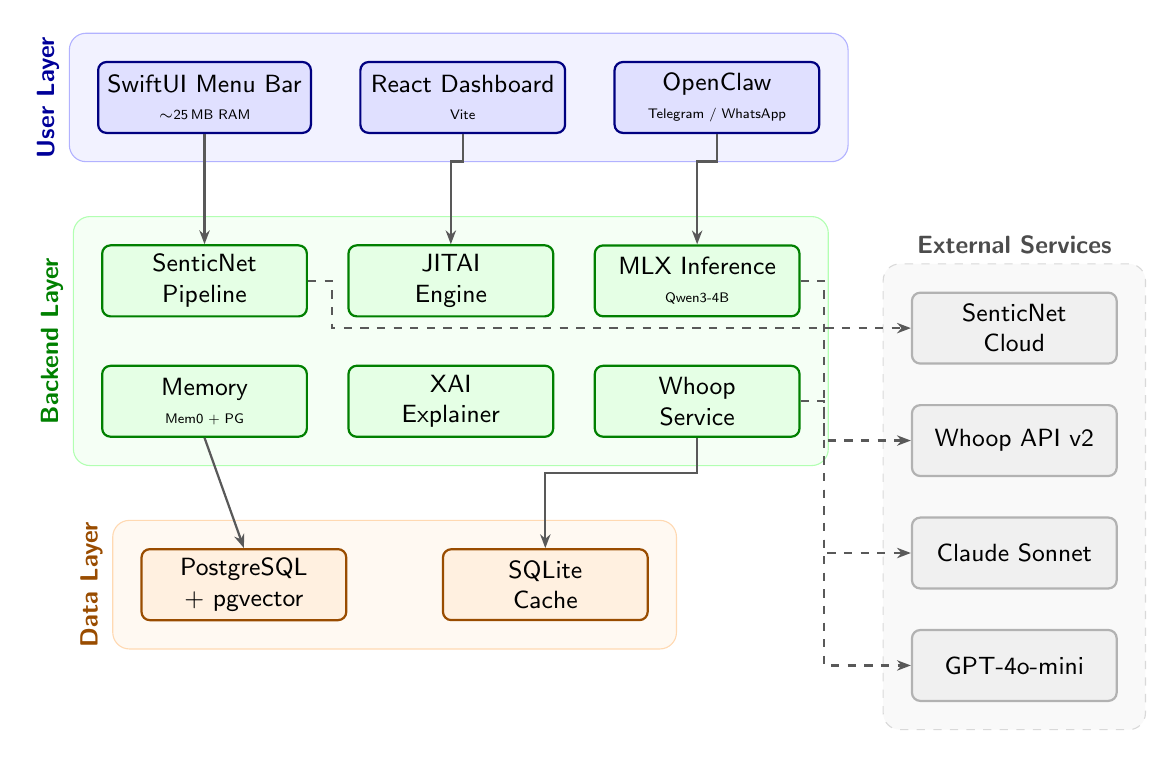
\begin{tikzpicture}[
    node distance=0.6cm and 0.5cm,
    every node/.style={font=\small},
    component/.style={
      rectangle, rounded corners=3pt, draw, thick,
      minimum width=2.6cm, minimum height=0.9cm,
      align=center, font=\small\sffamily
    },
    usercomp/.style={component, fill=blue!12, draw=blue!50!black},
    backcomp/.style={component, fill=green!10, draw=green!50!black},
    datacomp/.style={component, fill=orange!12, draw=orange!60!black},
    extcomp/.style={component, fill=gray!12, draw=gray!60},
    layerlabel/.style={font=\small\sffamily\bfseries, rotate=90, anchor=south},
    arr/.style={-{Stealth[length=5pt]}, thick, gray!70!black}
  ]
    % ── User Layer ──
    \node[usercomp] (swift) {SwiftUI Menu Bar\\[-1pt]{\tiny$\sim$25\,MB RAM}};
    \node[usercomp, right=0.6cm of swift] (react) {React Dashboard\\[-1pt]{\tiny Vite}};
    \node[usercomp, right=0.6cm of react] (openclaw) {OpenClaw\\[-1pt]{\tiny Telegram / WhatsApp}};

    % ── Backend Layer ──
    \node[backcomp, below=1.4cm of swift] (senticpipe) {SenticNet\\Pipeline};
    \node[backcomp, right=0.5cm of senticpipe] (jitai) {JITAI\\Engine};
    \node[backcomp, right=0.5cm of jitai] (mlx) {MLX Inference\\[-1pt]{\tiny Qwen3-4B}};
    \node[backcomp, below=0.6cm of senticpipe] (memory) {Memory\\[-1pt]{\tiny Mem0 + PG}};
    \node[backcomp, right=0.5cm of memory] (xai) {XAI\\Explainer};
    \node[backcomp, right=0.5cm of xai] (whoop) {Whoop\\Service};

    % ── Data Layer ──
    \node[datacomp, below=1.4cm of memory, xshift=0.5cm] (pg) {PostgreSQL\\+ pgvector};
    \node[datacomp, right=1.2cm of pg] (sqlite) {SQLite\\Cache};

    % ── External Services ──
    \node[extcomp, right=1.4cm of mlx, yshift=-0.6cm] (senticcloud) {SenticNet\\Cloud};
    \node[extcomp, below=0.5cm of senticcloud] (whoopapi) {Whoop API v2};
    \node[extcomp, below=0.5cm of whoopapi] (claude) {Claude Sonnet};
    \node[extcomp, below=0.5cm of claude] (gpt) {GPT-4o-mini};

    % ── Fit nodes for layer backgrounds ──
    \begin{scope}[on background layer]
      \node[fit=(swift)(react)(openclaw),
            fill=blue!5, draw=blue!30, rounded corners=6pt,
            inner sep=10pt, label={[layerlabel, blue!60!black]left:User Layer}] (userlayer) {};
      \node[fit=(senticpipe)(jitai)(mlx)(memory)(xai)(whoop),
            fill=green!4, draw=green!30, rounded corners=6pt,
            inner sep=10pt, label={[layerlabel, green!50!black]left:Backend Layer}] (backlayer) {};
      \node[fit=(pg)(sqlite),
            fill=orange!5, draw=orange!30, rounded corners=6pt,
            inner sep=10pt, label={[layerlabel, orange!60!black]left:Data Layer}] (datalayer) {};
      \node[fit=(senticcloud)(whoopapi)(claude)(gpt),
            fill=gray!5, draw=gray!30, rounded corners=6pt, dashed,
            inner sep=10pt, label={[font=\small\sffamily\bfseries, gray!60!black]above:External Services}] (extlayer) {};
    \end{scope}

    % ── Arrows: User -> Backend ──
    \draw[arr] (swift.south) -- ++(0,-0.35) -| (senticpipe.north);
    \draw[arr] (react.south) -- ++(0,-0.35) -| (jitai.north);
    \draw[arr] (openclaw.south) -- ++(0,-0.35) -| (mlx.north);

    % ── Arrows: Backend -> Data ──
    \draw[arr] (memory.south) -- (pg.north);
    \draw[arr] (whoop.south) -- ++(0,-0.45) -| (sqlite.north);

    % ── Arrows: Backend -> External ──
    \draw[arr, dashed] (senticpipe.east) -- ++(0.3,0) |- (senticcloud.west);
    \draw[arr, dashed] (whoop.east) -- ++(0.3,0) |- (whoopapi.west);
    \draw[arr, dashed] (mlx.east) -- ++(0.3,0) |- (claude.west);
    \draw[arr, dashed] (mlx.east) -- ++(0.3,0) |- (gpt.west);

  \end{tikzpicture}
  \caption{Three-layer system architecture of the ADHD Second Brain. The User Layer comprises a SwiftUI menu bar application, a React dashboard, and the OpenClaw interface. The Backend Layer hosts the FastAPI server (\texttt{localhost:8420}) with its constituent modules (${\sim}500$\,MB RAM $+$ ${\sim}2.3$\,GB GPU). The Data Layer combines PostgreSQL with pgvector and SQLite for persistent and vector-indexed storage. Dashed arrows indicate external service calls.}
  \label{fig:system_architecture}
\end{figure}

\textbf{User Layer.} The primary interface is a native macOS menu bar application built in SwiftUI ($\sim$25\,MB RAM), which polls screen metadata via the Accessibility API every two to three seconds and forwards it to the Backend Layer over local HTTP. A React dashboard (Vite) provides historical analytics and emotional trend visualisations, while OpenClaw offers a conversational interface for venting, task planning, and reflective journaling.

\textbf{Backend Layer.} Implemented as a FastAPI application on \texttt{localhost:8420}, the backend comprises six modules: (1)~the SenticNet Pipeline for affective analysis across thirteen APIs~\cite{cambria2024}; (2)~the JITAI Engine, evaluating behavioural metrics against Barkley's five executive function domains~\cite{barkley2010}; (3)~the Whoop Service for physiological data via OAuth~2.0; (4)~the MLX Inference module hosting Qwen3-4B at 4-bit precision on Apple Silicon; (5)~the Memory module coordinating Mem0 and PostgreSQL for semantic retrieval; and (6)~the XAI Explainer using a Concept Bottleneck Model for interpretable explanations. At steady state, the backend consumes $\sim$500\,MB RAM plus $\sim$2.3\,GB GPU memory.

\textbf{Data Layer.} PostgreSQL with pgvector provides combined relational and vector storage. Activity logs, emotional analyses, and conversation histories are stored relationally, while Mem0-generated embeddings are indexed via pgvector for sub-second semantic search. A lightweight SQLite database caches configuration state and transient metadata.

\textbf{External Services.} Four external services are used selectively: SenticNet Cloud (thirteen affective computing APIs)~\cite{cambria2024}, Whoop API~v2 (physiological metrics), Claude Sonnet (complex reasoning), and GPT-4o-mini (high-frequency classification and summarisation). A routing heuristic governs external LLM selection based on query complexity and latency requirements.

\textbf{Data Flows.} The architecture supports two data flows with distinct latency targets. The \emph{Hot Path} handles screen monitoring events within 100\,ms (activity classification, metric computation, SetFit emotion prediction, and intervention evaluation with emotion context). The \emph{Warm Path} handles conversational interactions within 3\,s (affective analysis, LLM generation, memory persistence). These are detailed in \Cref{sec:screen_monitoring} and \Cref{sec:affective_computing}; \Cref{fig:data_flows} illustrates both flows.

% --- MERMAID BACKUP ---
% flowchart LR
%   subgraph HotPath["Hot Path (<100ms)"]
%     direction TB
%     H1[Swift App] --> H2[Activity Classifier]
%     H2 --> H3[ADHD Metrics Engine]
%     H3 --> H3b[SetFit Emotion]
%     H3b --> H4[JITAI Engine]
%     H4 --> H5[Persist to PG]
%   end
%   subgraph WarmPath["Warm Path (<3s)"]
%     direction TB
%     W1[User Message] --> W2[Safety Check]
%     W2 --> W3[Emotion Analysis]
%     W3 --> W4[ADHD Signals]
%     W4 --> W5[LLM Generation]
%     W5 --> W6[Memory Store]
%   end
% --- END MERMAID ---

\begin{figure}[htbp]
  \centering
  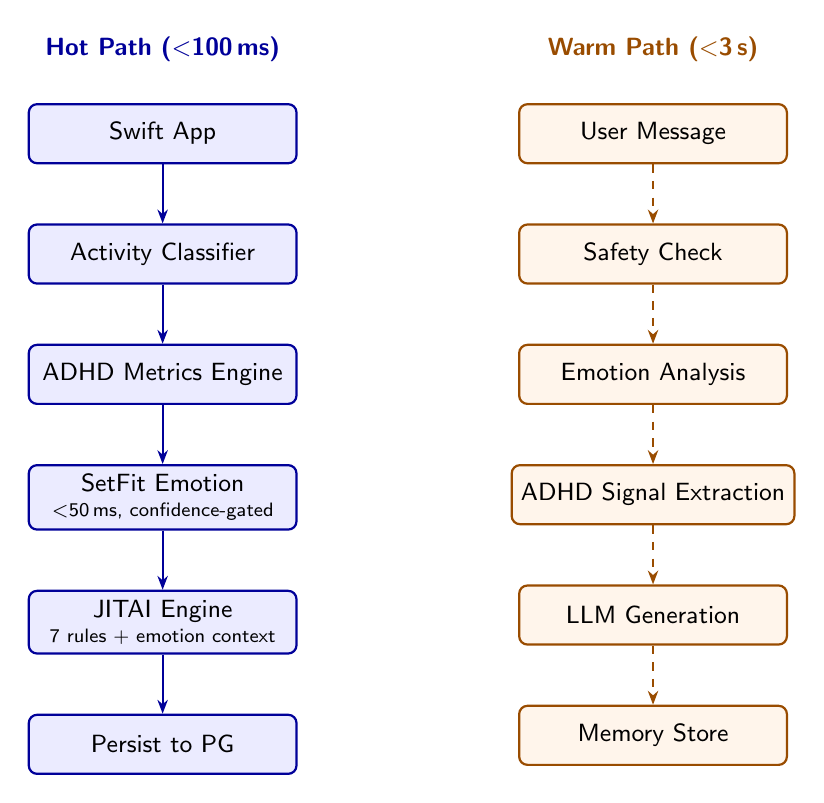
\begin{tikzpicture}[
    node distance=0.75cm,
    every node/.style={font=\small\sffamily},
    hotbox/.style={
      rectangle, rounded corners=3pt, draw=blue!60!black, thick,
      fill=blue!8, minimum width=3.4cm, minimum height=0.75cm, align=center
    },
    warmbox/.style={
      rectangle, rounded corners=3pt, draw=orange!60!black, thick,
      fill=orange!8, minimum width=3.4cm, minimum height=0.75cm, align=center
    },
    hotarr/.style={-{Stealth[length=5pt]}, thick, blue!60!black},
    warmarr/.style={-{Stealth[length=5pt]}, thick, orange!60!black, dashed}
  ]
    % ── Hot Path (left column) ──
    \node[hotbox] (h1) {Swift App};
    \node[hotbox, below=of h1] (h2) {Activity Classifier};
    \node[hotbox, below=of h2] (h3) {ADHD Metrics Engine};
    \node[hotbox, below=of h3] (h3b) {SetFit Emotion\\[-2pt]{\scriptsize $<$50\,ms, confidence-gated}};
    \node[hotbox, below=of h3b] (h4) {JITAI Engine\\[-2pt]{\scriptsize 7 rules + emotion context}};
    \node[hotbox, below=of h4] (h5) {Persist to PG};

    \draw[hotarr] (h1) -- (h2);
    \draw[hotarr] (h2) -- (h3);
    \draw[hotarr] (h3) -- (h3b);
    \draw[hotarr] (h3b) -- (h4);
    \draw[hotarr] (h4) -- (h5);

    % ── Warm Path (right column) ──
    \node[warmbox, right=2.8cm of h1] (w1) {User Message};
    \node[warmbox, below=of w1] (w2) {Safety Check};
    \node[warmbox, below=of w2] (w3) {Emotion Analysis};
    \node[warmbox, below=of w3] (w4) {ADHD Signal Extraction};
    \node[warmbox, below=of w4] (w5) {LLM Generation};
    \node[warmbox, below=of w5] (w6) {Memory Store};

    \draw[warmarr] (w1) -- (w2);
    \draw[warmarr] (w2) -- (w3);
    \draw[warmarr] (w3) -- (w4);
    \draw[warmarr] (w4) -- (w5);
    \draw[warmarr] (w5) -- (w6);

    % ── Path labels ──
    \node[above=0.4cm of h1, font=\small\sffamily\bfseries, blue!60!black]
      {Hot Path ($<$100\,ms)};
    \node[above=0.4cm of w1, font=\small\sffamily\bfseries, orange!60!black]
      {Warm Path ($<$3\,s)};

  \end{tikzpicture}
  \caption{Hot Path and Warm Path data flows. The Hot Path (solid arrows) processes screen monitoring events through activity classification, ADHD metrics computation, SetFit emotion prediction, and JITAI evaluation with confidence-gated emotion context within a 100\,ms budget. The Warm Path (dashed arrows) processes conversational input through safety checking, emotion analysis, LLM generation, and memory storage within a 3\,s budget.}
  \label{fig:data_flows}
\end{figure}


% =============================================================================
\section{Design Methodology}
\label{sec:design_methodology}
% =============================================================================

Development followed an agile, iterative methodology across nine implementation phases. This approach was selected because the system's reliance on multiple ML models demanded rapid prototyping cycles, and the interdependencies between affective computing accuracy, intervention timing, and user experience necessitated continuous cross-module integration testing. The phases established foundational infrastructure first (backend scaffolding, database schema), then layered intelligence progressively: screen monitoring, SenticNet integration, JITAI engine, on-device LLM inference, memory system, UI refinement, and end-to-end evaluation.

Four design principles governed all architectural decisions:

\begin{enumerate}[leftmargin=*, itemsep=4pt]
  \item \emph{Privacy by architecture}: raw screen captures and transcripts never leave the local machine; only anonymised metadata is sent externally when enrichment is required.
  \item \emph{Fail-fast over fail-safe}: components throw errors immediately rather than degrading silently---a deliberate choice for a pre-production system.
  \item \emph{Interpretability}: every decision is traceable to named concepts and explainable via the XAI module.
  \item \emph{Resource consciousness}: peak AI memory is constrained to 2.5\,GB with load-on-demand model instantiation for consumer Apple Silicon hardware.
\end{enumerate}

Each phase concluded with evaluation against predefined acceptance criteria: minimum accuracy thresholds for ML modules (e.g., 80\% weighted F1 for emotion classification) and latency percentile targets for real-time modules (e.g., p99~$<$~100\,ms for the Hot Path).


% =============================================================================
\section{On-Device LLM Module}
\label{sec:llm_module}
% =============================================================================

The On-Device LLM Module provides natural language understanding and generation without persistent cloud connectivity, ensuring that sensitive emotional disclosures remain on-device.

\textbf{Model Selection.} The module employs Qwen3-4B~\cite{yang2025}, selected after evaluating candidates against four criteria: parameter count compatible with consumer Apple Silicon, availability of 4-bit quantised weights, strong instruction-following performance relative to size, and MLX framework support. Qwen3-4B outperformed similarly-sized alternatives including Phi-3-mini and Llama-3.2-3B on the system's internal ADHD-relevant evaluation suite.

\textbf{Quantisation and Inference.} The model is quantised to 4-bit precision (GPTQ) via the MLX ecosystem~\cite{hannun2023}, reducing memory from $\sim$8\,GB (FP16) to $\sim$2.3\,GB while preserving over 95\% of full-precision accuracy. MLX exploits Apple Silicon's unified memory for zero-copy CPU--GPU data sharing, achieving 37.1 tokens/s on M-series chips. The model is memory-mapped on first use and evicted after a configurable idle timeout (default: 15~minutes), keeping the idle backend at $\sim$500\,MB. \Cref{tab:llm_performance} summarises performance characteristics.

\begin{table}[htbp]
  \centering
  \caption{On-device LLM performance characteristics for Qwen3-4B (4-bit quantised) on Apple Silicon via MLX.}
  \label{tab:llm_performance}
  \begin{tabular}{ll}
    \toprule
    \textbf{Metric} & \textbf{Value} \\
    \midrule
    Parameter count        & 4 billion \\
    Quantisation           & 4-bit (GPTQ) \\
    GPU memory footprint   & $\sim$2.3\,GB \\
    Inference throughput   & 37.1 tokens/s \\
    Time to first token    & $\sim$180\,ms \\
    Framework              & Apple MLX \\
    \bottomrule
  \end{tabular}
\end{table}

\textbf{Context Injection.} Before each invocation, the module constructs a structured prompt incorporating: (1)~the user's current emotional state from the SenticNet pipeline (\Cref{sec:affective_computing}), including classified emotion, polarity, and sarcasm detection; (2)~relevant long-term memories retrieved via Mem0 semantic search (\Cref{sec:memory_module}); and (3)~current screen activity context (active application, focus score, distraction ratio). This transforms the general-purpose model into an ADHD-aware agent that references historical patterns, current emotion, and task context.


% =============================================================================
\section{Affective Computing Module}
\label{sec:affective_computing}
% =============================================================================

The Affective Computing Module combines lexicon-based sentiment analysis with contrastive learning to understand the user's emotional state from text, operating along two axes: a multi-tier SenticNet orchestration pipeline and a custom SetFit-based emotion classifier.

\textbf{SenticNet Pipeline.} SenticNet~\cite{cambria2024} provides semantics-aware sentiment analysis grounded in the Hourglass of Emotions model~\cite{cambria2016}. The system orchestrates thirteen Cloud APIs in a four-tier cascade. Tier~1 (Safety) invokes depression detection, toxicity classification, and intensity estimation---if thresholds are exceeded, an emergency pathway is triggered immediately. Tier~2 (Core Emotional) performs emotion recognition, polarity detection, subjectivity analysis, and sarcasm detection. Tier~3 (ADHD Signals) extracts engagement, wellbeing, conceptual associations, and aspect-level sentiment. Tier~4 (Deep Analysis) performs personality profiling and ensemble aggregation, invoked only when preceding tiers yield conflicting signals. \Cref{fig:senticnet_pipeline} illustrates this cascade.

% --- MERMAID BACKUP ---
% flowchart TB
%   T1[Tier 1: Safety<br>Depression + Toxicity + Intensity] -->|Pass| T2
%   T1 -->|Threshold exceeded| EM[Emergency Response]
%   T2[Tier 2: Core Emotional<br>Emotion + Polarity + Subjectivity + Sarcasm] --> T3
%   T3[Tier 3: ADHD Signals<br>Engagement + Wellbeing + Concepts + Aspects] --> T4
%   T4[Tier 4: Deep Analysis<br>Personality + Ensemble]
%   style T1 fill:#fee,stroke:#c00
%   style T2 fill:#ffe,stroke:#c80
%   style T3 fill:#efe,stroke:#080
%   style T4 fill:#eef,stroke:#008
%   style EM fill:#fcc,stroke:#c00
% --- END MERMAID ---

\begin{figure}[htbp]
  \centering
  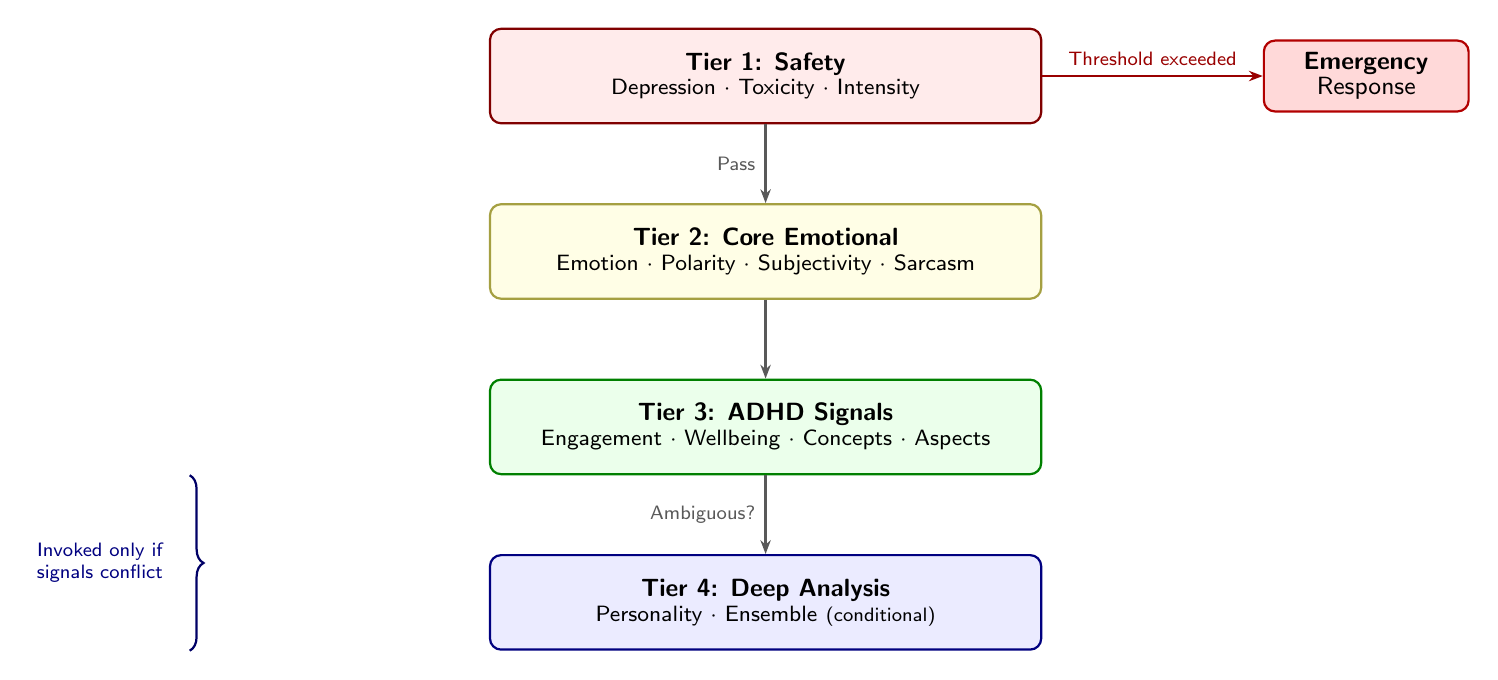
\begin{tikzpicture}[
    node distance=1.0cm,
    every node/.style={font=\small\sffamily},
    tierbox/.style={
      rectangle, rounded corners=4pt, draw, thick,
      minimum width=7cm, minimum height=1.2cm, align=center
    },
    tier1/.style={tierbox, fill=red!8, draw=red!50!black},
    tier2/.style={tierbox, fill=yellow!10, draw=yellow!60!black},
    tier3/.style={tierbox, fill=green!8, draw=green!50!black},
    tier4/.style={tierbox, fill=blue!8, draw=blue!50!black},
    emergency/.style={
      rectangle, rounded corners=4pt, draw=red!70!black, thick,
      fill=red!15, minimum width=2.6cm, minimum height=0.9cm, align=center
    },
    downarr/.style={-{Stealth[length=5pt]}, thick, gray!70!black},
    emergarr/.style={-{Stealth[length=5pt]}, thick, red!60!black}
  ]
    \node[tier1] (t1) {%
      \textbf{Tier 1: Safety}\\[-2pt]
      {\footnotesize Depression $\cdot$ Toxicity $\cdot$ Intensity}};
    \node[tier2, below=of t1] (t2) {%
      \textbf{Tier 2: Core Emotional}\\[-2pt]
      {\footnotesize Emotion $\cdot$ Polarity $\cdot$ Subjectivity $\cdot$ Sarcasm}};
    \node[tier3, below=of t2] (t3) {%
      \textbf{Tier 3: ADHD Signals}\\[-2pt]
      {\footnotesize Engagement $\cdot$ Wellbeing $\cdot$ Concepts $\cdot$ Aspects}};
    \node[tier4, below=of t3] (t4) {%
      \textbf{Tier 4: Deep Analysis}\\[-2pt]
      {\footnotesize Personality $\cdot$ Ensemble} {\scriptsize (conditional)}};

    % Emergency branch
    \node[emergency, right=2.8cm of t1] (emerg) {\textbf{Emergency}\\[-2pt]Response};

    % Vertical arrows
    \draw[downarr] (t1.south) -- node[left, font=\scriptsize\sffamily, text=gray!70!black]{Pass} (t2.north);
    \draw[downarr] (t2.south) -- (t3.north);
    \draw[downarr] (t3.south) -- node[left, font=\scriptsize\sffamily, text=gray!70!black]{Ambiguous?} (t4.north);

    % Emergency arrow
    \draw[emergarr] (t1.east) -- node[above, font=\scriptsize\sffamily, text=red!60!black]{Threshold exceeded} (emerg.west);

    % Conditional annotation for Tier 4
    \draw[decorate, decoration={brace, amplitude=5pt, mirror}, thick, blue!40!black]
      ([xshift=-3.8cm]t4.south west) -- ([xshift=-3.8cm]t3.south west)
      node[midway, left=6pt, font=\scriptsize\sffamily, text=blue!50!black, align=right]
      {Invoked only if\\signals conflict};

  \end{tikzpicture}
  \caption{Four-tier SenticNet orchestration pipeline. Each tier is evaluated sequentially; Tier~1 may short-circuit to an emergency pathway if safety thresholds are exceeded. Tier~4 is invoked conditionally based on signal ambiguity in Tiers~2 and~3.}
  \label{fig:senticnet_pipeline}
\end{figure}

\textbf{Emotion Taxonomy.} Rather than adopting a general-purpose taxonomy such as Ekman's six basic emotions, the system defines six ADHD-specific categories: \emph{joyful}, \emph{focused}, \emph{frustrated}, \emph{anxious}, \emph{disengaged}, and \emph{overwhelmed}. This taxonomy was developed from ADHD literature~\cite{barkley2010, diamond2013} and reflects emotional states most salient to executive function regulation. \emph{Focused} and \emph{disengaged} correspond to attentional states central to ADHD symptomatology, while \emph{overwhelmed} captures executive overload preceding task abandonment.

\textbf{SetFit Emotion Classifier.} The classifier employs a contrastive learning framework inspired by SetFit~\cite{reimers2019}, implemented manually due to library incompatibilities with the project's transformer versions. The base encoder is \texttt{all-mpnet-base-v2}~\cite{wang2020}, a 110M-parameter sentence transformer. Training uses CoSENT loss over all unique pairs including hard negatives from adjacent categories (e.g., \emph{anxious}--\emph{overwhelmed}). With 210 manually curated sentences, a single epoch achieves 86\% weighted F1---superior to two epochs (84\%), indicating overfitting. Augmenting with 288 LLM-generated sentences degraded performance to 82\% due to distributional shift and class imbalance. \Cref{tab:emotion_classifiers} summarises results.

\begin{table}[htbp]
  \centering
  \caption{Emotion classifier accuracy comparison across approaches. Weighted F1 scores are reported on a held-out test set of 50 manually labelled sentences.}
  \label{tab:emotion_classifiers}
  \begin{tabular}{lcc}
    \toprule
    \textbf{Approach} & \textbf{Training Data} & \textbf{Weighted F1} \\
    \midrule
    Baseline SenticNet             & ---              & 0.28 \\
    Hybrid (Embedding + SenticNet) & 210 sentences    & 0.74 \\
    DistilBERT fine-tuned          & 210 sentences    & 0.62 \\
    DistilBERT fine-tuned          & 1,200 augmented  & 0.72 \\
    SetFit (CoSENT, 1 epoch)       & 210 sentences    & \textbf{0.86} \\
    SetFit (CoSENT, 1 epoch)       & 498 sentences    & 0.82 \\
    \bottomrule
  \end{tabular}
\end{table}

\textbf{SetFit-to-PASE Mapping for Emotion Radar.} To bridge the gap between SetFit's categorical labels and the dashboard's four-axis Emotion Radar, each SetFit label is mapped to a canonical PASE (Pleasantness, Attention, Sensitivity, Aptitude) profile. These profiles encode the typical emotional geometry of each ADHD state---for example, \emph{frustrated} maps to low pleasantness (0.15), moderate attention (0.40), high sensitivity (0.80), and low aptitude (0.30). A confidence-weighted blending function interpolates between the canonical profile and a neutral centre (all~0.5) proportional to SetFit's confidence score, ensuring that low-confidence predictions do not produce misleading radar shapes. This approach was selected over direct SenticNet Hourglass scoring because SenticNet's concept-level analysis produces unreliable values on short, informal text such as window titles.

\textbf{Concept Bottleneck Model for Explainability.} The emotion classifier is wrapped in a Concept Bottleneck Model (CBM)~\cite{koh2020} to satisfy the interpretability principle. The CBM first predicts intermediate human-interpretable concepts---such as ``frustration with task switching'' or ``anxiety about deadlines''---then derives the emotion label from these concepts. This enables explanations of the form: ``You appear \emph{overwhelmed} because the system detected high task-switching frequency and negative polarity toward the current assignment.'' Such explanations support metacognitive awareness, a known protective factor in ADHD self-regulation~\cite{diamond2013}.


% =============================================================================
\section{Memory and Context Module}
\label{sec:memory_module}
% =============================================================================

The Memory and Context Module provides longitudinal awareness of the user's behavioural patterns, emotional history, and conversational context, transforming the system from stateless to personalised.

\textbf{Mem0 Integration.} Mem0~\cite{chhikara2025} serves as the primary memory abstraction, automatically extracting salient facts from conversations and storing them as structured entries with metadata. In evaluation, Mem0 demonstrated a 26\% improvement in retrieval relevance over the OpenAI memory baseline, as measured by Mean Reciprocal Rank on ADHD-specific recall queries. This advantage stems from Mem0's graph-based memory organisation capturing relational structure.

\textbf{PostgreSQL + pgvector.} Memory embeddings are persisted via the pgvector extension for approximate nearest-neighbour search. The embedding model is \texttt{all-mpnet-base-v2}---shared with the emotion classifier for representational consistency. At query time, cosine similarity search retrieves the top-$k$ relevant memories for injection into the LLM prompt (\Cref{sec:llm_module}).

\textbf{Semantic Retrieval Pipeline.} The retrieval pipeline comprises three stages: (1)~encoding the user input via the shared sentence transformer, (2)~pgvector cosine similarity search over the memory index, and (3)~re-ranking by temporal recency and contextual relevance. \Cref{fig:memory_pipeline} illustrates this pipeline.

% --- MERMAID BACKUP ---
% flowchart LR
%   A[User Input] --> B[Encode<br>all-mpnet-base-v2]
%   B --> C[pgvector Search<br>Cosine Similarity]
%   C --> D[Re-rank<br>Temporal + Context]
%   D --> E[Inject into<br>LLM Prompt]
% --- END MERMAID ---

\begin{figure}[htbp]
  \centering
  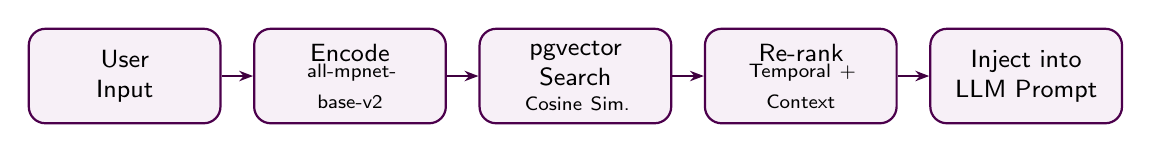
\begin{tikzpicture}[
    node distance=0.4cm,
    every node/.style={font=\small\sffamily},
    pipebox/.style={
      rectangle, rounded corners=6pt, draw=violet!60!black, thick,
      fill=violet!6, minimum width=2.4cm, minimum height=1.2cm, align=center,
      text width=2.2cm
    },
    arr/.style={-{Stealth[length=5pt]}, thick, violet!50!black}
  ]
    \node[pipebox] (input) {User\\Input};
    \node[pipebox, right=of input] (encode) {Encode\\[-2pt]{\scriptsize all-mpnet-\\base-v2}};
    \node[pipebox, right=of encode] (search) {pgvector\\Search\\[-2pt]{\scriptsize Cosine Sim.}};
    \node[pipebox, right=of search] (rerank) {Re-rank\\[-2pt]{\scriptsize Temporal +\\Context}};
    \node[pipebox, right=of rerank] (inject) {Inject into\\LLM Prompt};

    \draw[arr] (input) -- (encode);
    \draw[arr] (encode) -- (search);
    \draw[arr] (search) -- (rerank);
    \draw[arr] (rerank) -- (inject);
  \end{tikzpicture}
  \caption{Semantic memory retrieval pipeline. User input is encoded via the shared sentence transformer, matched against the pgvector index by cosine similarity, and re-ranked by temporal recency and activity context before injection into the LLM prompt.}
  \label{fig:memory_pipeline}
\end{figure}


% =============================================================================
\section{Screen Monitoring Module}
\label{sec:screen_monitoring}
% =============================================================================

The Screen Monitoring Module implements the Hot Path, continuously observing desktop activity and computing real-time ADHD-relevant behavioural metrics to trigger just-in-time interventions.

\textbf{Screen Capture.} The SwiftUI application polls active window metadata every two to three seconds via the macOS Accessibility API, capturing the application name, window title, and browser tab URL where available. Only metadata is captured---not pixel-level screenshots---preserving privacy while providing sufficient signal for classification.

\textbf{Activity Classifier.} A four-level hierarchical rule-based classifier resolves activity categories with minimal cost, resorting to expensive methods only when simpler levels fail. Level~1 matches the application name against a curated dictionary; Level~2 matches browser URL domains; Level~3 applies keyword matching to window titles; Level~4 routes unresolved metadata to the on-device embedding model. Levels~1--3 execute in under 5\,ms and resolve 78\% of events; Level~4 ($\sim$8\,ms) handles the remaining 22\%. \Cref{fig:activity_classifier} illustrates this cascade.

% --- MERMAID BACKUP ---
% flowchart TB
%   IN[Screen Event] --> L1{L1: App Name?}
%   L1 -->|56.5% resolved| OUT[Classification Result]
%   L1 -->|No match| L2{L2: URL Domain?}
%   L2 -->|Match| OUT
%   L2 -->|No match| L3{L3: Title Keywords?}
%   L3 -->|21.5% resolved| OUT
%   L3 -->|No match| L4{L4: Embedding}
%   L4 -->|22% resolved| OUT
% --- END MERMAID ---

\begin{figure}[htbp]
  \centering
  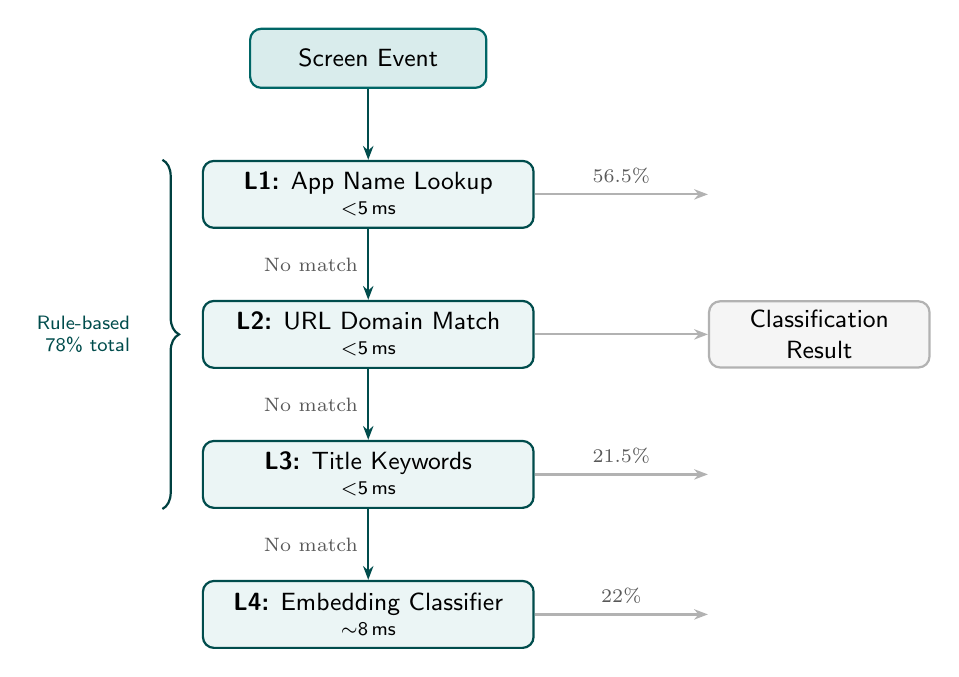
\begin{tikzpicture}[
    node distance=0.9cm,
    every node/.style={font=\small\sffamily},
    levelbox/.style={
      rectangle, rounded corners=4pt, draw=teal!60!black, thick,
      fill=teal!8, minimum width=4.2cm, minimum height=0.85cm, align=center
    },
    resultbox/.style={
      rectangle, rounded corners=4pt, draw=gray!60, thick,
      fill=gray!8, minimum width=2.8cm, minimum height=0.75cm, align=center
    },
    inputbox/.style={
      rectangle, rounded corners=4pt, draw=teal!80!black, thick,
      fill=teal!15, minimum width=3.0cm, minimum height=0.75cm, align=center
    },
    downarr/.style={-{Stealth[length=5pt]}, thick, teal!60!black},
    resarr/.style={-{Stealth[length=5pt]}, thick, gray!60}
  ]
    \node[inputbox] (input) {Screen Event};
    \node[levelbox, below=of input] (l1) {\textbf{L1:} App Name Lookup\\[-2pt]{\scriptsize $<$5\,ms}};
    \node[levelbox, below=of l1] (l2) {\textbf{L2:} URL Domain Match\\[-2pt]{\scriptsize $<$5\,ms}};
    \node[levelbox, below=of l2] (l3) {\textbf{L3:} Title Keywords\\[-2pt]{\scriptsize $<$5\,ms}};
    \node[levelbox, below=of l3] (l4) {\textbf{L4:} Embedding Classifier\\[-2pt]{\scriptsize $\sim$8\,ms}};

    % Result node
    \node[resultbox, right=2.2cm of l2] (result) {Classification\\Result};

    % Vertical flow
    \draw[downarr] (input) -- (l1);
    \draw[downarr] (l1) -- node[left, font=\scriptsize, text=gray!70!black]{No match} (l2);
    \draw[downarr] (l2) -- node[left, font=\scriptsize, text=gray!70!black]{No match} (l3);
    \draw[downarr] (l3) -- node[left, font=\scriptsize, text=gray!70!black]{No match} (l4);

    % Resolution arrows with labels
    \draw[resarr] (l1.east) -- node[above, font=\scriptsize, text=gray!70!black]{56.5\%} (result.west |- l1.east);
    \draw[resarr] (l2.east) -- node[above, font=\scriptsize, text=gray!70!black]{} (result.west |- l2.east);
    \draw[resarr] (l3.east) -- node[above, font=\scriptsize, text=gray!70!black]{21.5\%} (result.west |- l3.east);
    \draw[resarr] (l4.east) -- node[above, font=\scriptsize, text=gray!70!black]{22\%} (result.west |- l4.east);

    % Brace for rule-based
    \draw[decorate, decoration={brace, amplitude=6pt}, thick, teal!50!black]
      ([xshift=-0.5cm]l1.north west) -- ([xshift=-0.5cm]l3.south west)
      node[midway, left=8pt, font=\scriptsize\sffamily, text=teal!60!black, align=right]
      {Rule-based\\78\% total};

  \end{tikzpicture}
  \caption{Four-level hierarchical activity classifier. Each level is attempted in sequence; classification terminates at the first level that produces a confident result. Levels~1--3 are rule-based and resolve 78\% of events in under 5\,ms. Level~4 (embedding fallback) is invoked for the remaining 22\%.}
  \label{fig:activity_classifier}
\end{figure}

\textbf{ADHD Metrics Engine.} Classified events feed into an in-memory metrics engine computing four real-time indicators: (1)~\emph{context switch rate} (application transitions per unit time), (2)~\emph{focus score} (sustained engagement with a task-relevant application), (3)~\emph{distraction ratio} (proportion of time in non-task-relevant applications within a sliding window), and (4)~\emph{streak} (uninterrupted focus duration). Each update requires less than 1\,ms.


% =============================================================================
\section{Intervention System Design}
\label{sec:intervention_system}
% =============================================================================

The Intervention System implements a Just-In-Time Adaptive Intervention (JITAI) framework grounded in Barkley's five executive function domains: inhibition, working memory, emotional self-regulation, self-motivation, and planning/problem-solving~\cite{barkley2010}. Informed by Diamond's EF development framework~\cite{diamond2013}, the system delivers targeted micro-interventions at moments of detected executive dysfunction.

\textbf{JITAI Engine.} The engine consumes real-time metrics from the ADHD Metrics Engine (\Cref{sec:screen_monitoring}) and a confidence-gated emotion context from the SetFit classifier (\Cref{sec:affective_computing}), evaluating seven intervention rules associated with each EF domain in under 2\,ms. The seven rules span four EF domains: Rule~1 targets distraction spirals (self-restraint); Rule~2 targets sustained disengagement (self-motivation); Rule~3 targets hyperfocus on the wrong task (self-management of time); and Rules~4a--4d target emotion-driven states (self-regulation of emotion and self-motivation). Rules~4a--4d are enabled by SetFit predictions wired through the screen activity hot path: Rule~4a fires on \emph{overwhelmed} states (emotional escalation), Rule~4b on \emph{frustrated} combined with high context-switching (frustration spiral), Rule~4c on \emph{anxious} combined with high distraction (anxiety distraction), and Rule~4d on persistent \emph{disengaged} states exceeding 10~minutes (emotion disengagement). Each emotion-based rule is gated by SetFit confidence---thresholds of 0.7 for overwhelmed, frustrated, and anxious, and 0.6 for disengaged---to prevent false-positive interruptions that would be particularly disruptive for ADHD users.

\textbf{Thompson Sampling for Personalisation.} Because ADHD symptom profiles are heterogeneous, the engine employs Thompson Sampling---a Bayesian bandit algorithm---to learn which intervention types are most effective per user. Each type maintains a Beta distribution updated by observed successes and failures, converging over time to preferentially select high-efficacy interventions. \Cref{fig:jitai_loop} illustrates the complete evaluation and personalisation loop.

% --- MERMAID BACKUP ---
% flowchart TB
%   A[Real-Time Metrics<br>Context switches, Focus, Distraction] --> B[EF Domain Evaluation<br>5 Barkley domains]
%   C[Emotional State<br>From SenticNet Pipeline] --> B
%   B --> D{Intervention<br>Warranted?}
%   D -->|No| E[Continue Monitoring]
%   D -->|Yes| F[Thompson Sampling<br>Sample Beta distributions]
%   F --> G[Select Intervention Type]
%   G --> H[Deliver via Tier 1-4]
%   H --> I[Observe User Response]
%   I --> J[Update Beta Parameters]
%   J --> F
% --- END MERMAID ---

\begin{figure}[htbp]
  \centering
  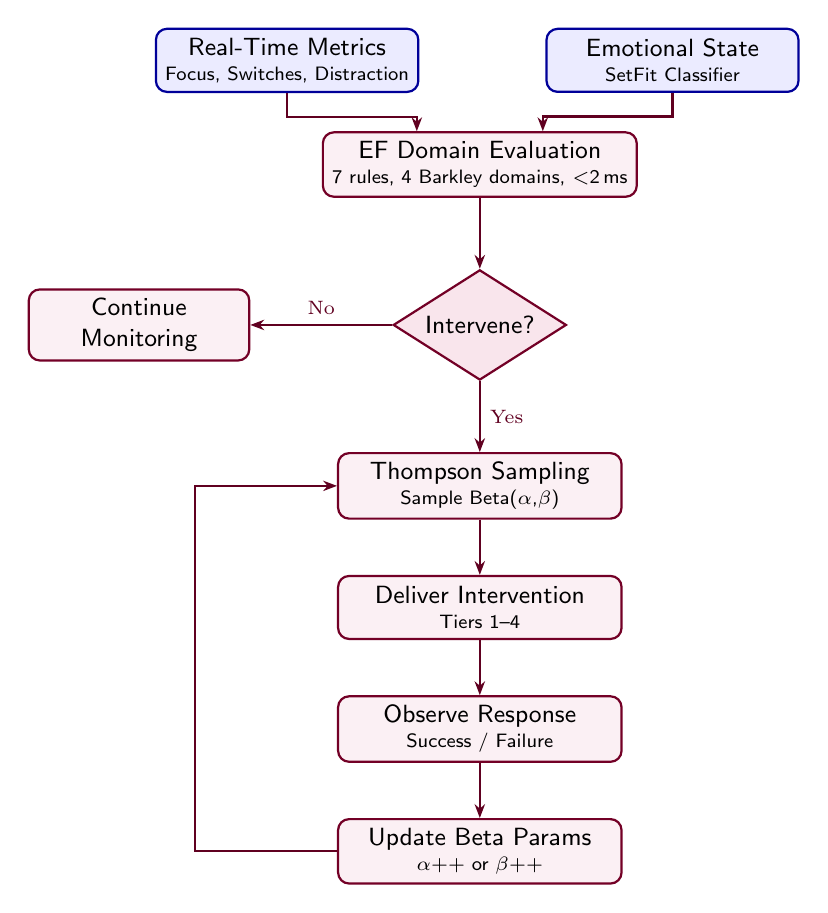
\begin{tikzpicture}[
    node distance=0.8cm and 0.8cm,
    every node/.style={font=\small\sffamily},
    procbox/.style={
      rectangle, rounded corners=4pt, draw=purple!60!black, thick,
      fill=purple!6, minimum width=3.6cm, minimum height=0.8cm, align=center
    },
    inputbox/.style={
      rectangle, rounded corners=4pt, draw=blue!60!black, thick,
      fill=blue!8, minimum width=3.2cm, minimum height=0.8cm, align=center
    },
    decbox/.style={
      diamond, draw=purple!60!black, thick, fill=purple!10,
      minimum width=2.2cm, minimum height=1.4cm, align=center,
      inner sep=1pt, aspect=1.8
    },
    arr/.style={-{Stealth[length=5pt]}, thick, purple!50!black}
  ]
    % Inputs
    \node[inputbox] (metrics) {Real-Time Metrics\\[-2pt]{\scriptsize Focus, Switches, Distraction}};
    \node[inputbox, right=1.6cm of metrics] (emotion) {Emotional State\\[-2pt]{\scriptsize SetFit Classifier}};

    % EF Evaluation
    \node[procbox, below=0.9cm of $(metrics)!0.5!(emotion)$] (eval) {EF Domain Evaluation\\[-2pt]{\scriptsize 7 rules, 4 Barkley domains, $<$2\,ms}};

    % Decision
    \node[decbox, below=0.9cm of eval] (decide) {Intervene?};

    % No branch
    \node[procbox, left=1.8cm of decide, minimum width=2.8cm] (cont) {Continue\\Monitoring};

    % Thompson Sampling branch
    \node[procbox, below=0.9cm of decide] (thompson) {Thompson Sampling\\[-2pt]{\scriptsize Sample Beta($\alpha$,$\beta$)}};
    \node[procbox, below=0.7cm of thompson] (deliver) {Deliver Intervention\\[-2pt]{\scriptsize Tiers 1--4}};
    \node[procbox, below=0.7cm of deliver] (observe) {Observe Response\\[-2pt]{\scriptsize Success / Failure}};
    \node[procbox, below=0.7cm of observe] (update) {Update Beta Params\\[-2pt]{\scriptsize $\alpha{+}{+}$ or $\beta{+}{+}$}};

    % Arrows from inputs to EF evaluation
    \draw[arr] (metrics.south) -- ++(0,-0.3) -| ([xshift=-0.8cm]eval.north);
    \draw[arr] (emotion.south) -- ++(0,-0.3) -| ([xshift=0.8cm]eval.north);
    \draw[arr] (eval) -- (decide);
    \draw[arr] (decide.west) -- node[above, font=\scriptsize]{No} (cont.east);
    \draw[arr] (decide.south) -- node[right, font=\scriptsize]{Yes} (thompson.north);
    \draw[arr] (thompson) -- (deliver);
    \draw[arr] (deliver) -- (observe);
    \draw[arr] (observe) -- (update);

    % Feedback loop
    \draw[arr] (update.west) -- ++(-1.8,0) |- (thompson.west);

  \end{tikzpicture}
  \caption{JITAI evaluation and personalisation loop. Real-time metrics and confidence-gated SetFit emotion context feed into the seven-rule executive function evaluation across four Barkley domains. When intervention is warranted, Thompson Sampling selects the intervention type, and user responses update the Beta distribution parameters for subsequent decisions.}
  \label{fig:jitai_loop}
\end{figure}

\textbf{Multi-Tier Intervention Delivery.} Interventions follow a four-tier escalation ladder (\Cref{tab:intervention_tiers}), proceeding to higher tiers only if lower ones fail to restore focus within a configurable observation window.

\begin{table}[htbp]
  \centering
  \caption{Multi-tier intervention escalation ladder with triggering conditions and delivery mechanisms.}
  \label{tab:intervention_tiers}
  \begin{tabular}{llll}
    \toprule
    \textbf{Tier} & \textbf{Type} & \textbf{Trigger Condition} & \textbf{Delivery Mechanism} \\
    \midrule
    1 & Nudge   & Mild metric deviation       & Menu bar indicator \\
    2 & Popup   & Sustained metric deviation   & macOS notification \\
    3 & Overlay & Escalation from Tier~2       & Semi-transparent overlay \\
    4 & Block   & Escalation from Tier~3       & Application restriction \\
    \bottomrule
  \end{tabular}
\end{table}


% =============================================================================
\section{UI/UX Design}
\label{sec:uiux_design}
% =============================================================================

The user interface comprises two complementary surfaces. The SwiftUI menu bar application provides an always-available, minimal-footprint entry point displaying current focus score, emotional state, and streak duration, with access to the OpenClaw conversational interface. It follows macOS Human Interface Guidelines to minimise cognitive overhead---critical for users with ADHD, who are disproportionately affected by interface complexity~\cite{beattie2025}.

The React dashboard provides a richer analytical interface for historical trends, emotional trajectories, and intervention efficacy over configurable time windows. Both interfaces employ ADHD-informed design: minimal visual clutter, high-contrast colour coding (green/amber/red for focus states), and progressive disclosure. Intervention notifications are non-punitive and action-oriented, framed positively to avoid triggering rejection-sensitive dysphoria.


% =============================================================================
\section{Technology Stack Selection}
\label{sec:tech_stack}
% =============================================================================

\Cref{tab:tech_stack} presents the technology stack with selection justifications, governed by on-device deployment compatibility, Python ML ecosystem integration, and Apple Silicon real-time processing suitability.

\begin{table}[htbp]
  \centering
  \caption{Technology stack selection with justifications.}
  \label{tab:tech_stack}
  \begin{tabular}{p{2.8cm}p{3.8cm}p{7cm}}
    \toprule
    \textbf{Component} & \textbf{Technology} & \textbf{Justification} \\
    \midrule
    Backend framework & FastAPI (Python~3.11) & Native async support; direct access to the Python ML ecosystem (PyTorch, Transformers, scikit-learn); automatic OpenAPI documentation generation \\
    \addlinespace
    Database & PostgreSQL + pgvector & Combined relational and vector storage eliminates the need for a separate vector database; mature ACID guarantees for activity logs; pgvector supports IVFFlat and HNSW indexing for sub-millisecond ANN search \\
    \addlinespace
    On-device LLM & Qwen3-4B via MLX & 4-bit quantisation fits within 2.5\,GB GPU budget; MLX exploits Apple Silicon unified memory for zero-copy inference; 37.1\,tok/s throughput enables interactive conversation \\
    \addlinespace
    Affective computing & SenticNet + SetFit & SenticNet provides interpretable, multi-dimensional affective features grounded in the Hourglass of Emotions~\cite{cambria2016}; SetFit achieves 86\% F1 with only 210 training sentences via contrastive learning \\
    \addlinespace
    Sentence encoder & all-mpnet-base-v2 & State-of-the-art sentence embeddings on STS benchmarks~\cite{reimers2019}; shared across emotion classification and memory retrieval for representational consistency \\
    \addlinespace
    Memory & Mem0 & 26\% retrieval relevance improvement over OpenAI memory baseline~\cite{chhikara2025}; graph-based memory organisation captures relational structure \\
    \addlinespace
    Desktop client & SwiftUI & Native macOS integration; direct access to Accessibility API for screen metadata capture; minimal resource footprint ($\sim$25\,MB RAM) \\
    \addlinespace
    Dashboard & React + Vite & Component-based architecture suits modular analytics views; Vite provides sub-second hot module replacement during development \\
    \bottomrule
  \end{tabular}
\end{table}

FastAPI was selected over Flask and Django for its native asynchronous request handling, essential for concurrent screen monitoring and conversational requests. Python~3.11 was chosen for compatibility with required ML packages (Transformers~5.3.0, sentence-transformers~5.2.3, PyTorch~2.10.0, scikit-learn~1.7.2). LoRA~\cite{hu2022} and QLoRA~\cite{dettmers2023} were evaluated for future model adaptation but not employed, as Qwen3-4B with prompt engineering proved sufficient. Emerging agentic RAG work~\cite{lin2025, xu2024} informed the memory retrieval design, though the current implementation uses a simpler three-stage pipeline.

\bigskip

This concludes the system design chapter. The three-layer architecture, dual data-flow model, and modular decomposition provide the structural foundation for implementation (Chapter~4) and evaluation (Chapter~5).

% =============================================================================
% Chapter 4 — Implementation
% =============================================================================
\chapter{Implementation}
\label{ch:implementation}

This chapter presents the implementation of each module in the ADHD Second Brain system, organised bottom-up: development environment (\cref{sec:dev-environment}), LLM inference (\cref{sec:llm-pipeline}), emotion classification (\cref{sec:emotion-pipeline}), SenticNet affective computing (\cref{sec:senticnet-pipeline}), persistent memory (\cref{sec:memory-system}), screen monitoring (\cref{sec:screen-monitoring}), the intervention engine (\cref{sec:intervention-engine}), client applications (\cref{sec:client-applications}), and implementation challenges (\cref{sec:implementation-challenges}).

% -----------------------------------------------------------------------------
\section{Development Environment and Tools}
\label{sec:dev-environment}

% .............................................................................
\subsection{Hardware and Runtime Environment}
\label{subsec:hardware-runtime}

All development, training, and evaluation were conducted on a MacBook Pro with the Apple M4 chip and 16\,GB of unified memory. The M4's unified memory architecture allows the GPU and CPU to share physical memory without explicit transfers, which the MLX framework \cite{hannun2023} exploits to dispatch LLM inference kernels to the GPU without host-to-device copy overhead. The 16\,GB budget imposes a hard constraint: the quantised LLM (2.3\,GB), sentence transformer (420\,MB), SenticNet cache, pgvector index, and Python runtime must coexist within this envelope, motivating the load-on-demand architecture described in \cref{subsec:model-selection}.

% .............................................................................
\subsection{Core Libraries and Frameworks}
\label{subsec:core-libraries}

The Python runtime was pinned to version 3.11 after Python 3.14 introduced breaking \texttt{importlib} changes that caused failures in \texttt{torch}, \texttt{transformers}, and \texttt{sentence-transformers}. The core ML stack comprises \texttt{transformers} 5.3.0 \cite{yang2025}, \texttt{sentence-transformers} 5.2.3 \cite{reimers2019}, PyTorch 2.10.0, and scikit-learn 1.7.2. The \texttt{setfit} library was rejected due to a broken dependency on \texttt{default\_logdir} removed in \texttt{transformers} 5.x; the contrastive training loop was instead implemented manually using \texttt{sentence-transformers} and PyTorch, as detailed in \cref{subsec:approach-b}.

% .............................................................................
\subsection{Data Infrastructure and Build Automation}
\label{subsec:data-infrastructure}

The data layer runs PostgreSQL 16 with the \texttt{pgvector} extension via Docker Compose, providing vector similarity search with cosine distance for the Mem0 memory framework \cite{chhikara2025}. Build automation uses a Makefile: \texttt{make test} runs the full suite of over 330 tests, \texttt{make bench} executes performance benchmarks, and \texttt{make all-eval} runs all evaluation pipelines including the comparative analysis reported in \cref{ch:testing-evaluation}.

% .............................................................................
\subsection{Version Control and Dependency Management}
\label{subsec:version-control}

Dependencies are pinned in \texttt{requirements.txt} with exact version specifiers. The technology stack spans Python 3.11 (AI/ML backend via FastAPI), Swift 5.9 (native macOS menu bar application and screen monitoring), and TypeScript (React web dashboard). Integration between Swift and Python occurs via HTTP at localhost, with JSON payloads defined by shared schema specifications.

% -----------------------------------------------------------------------------
\section{LLM Inference Pipeline}
\label{sec:llm-pipeline}

% .............................................................................
\subsection{On-Device Model Selection and Quantisation}
\label{subsec:model-selection}

After evaluating Phi-3-mini (3.8B), Llama-3.2-3B, and Gemma-2-2B, Qwen3-4B \cite{yang2025} was selected for its native dual-mode generation (\texttt{/think} and \texttt{/no\_think}). Applying 4-bit GPTQ quantisation via MLX reduces memory from 8\,GB (FP16) to 2.3\,GB, a 71\% reduction, following the principles of Dettmers et al.\ \cite{dettmers2023}. The pre-quantised model is obtained from the MLX Community repository on Hugging Face Hub.

The model uses a load-on-demand pattern with a weak reference cache. When a coaching response is requested, the system checks whether the model is resident via \texttt{weakref.ref}; if garbage-collected, it is reloaded from disk in 0.94 seconds. This ensures the LLM does not permanently occupy 2.3\,GB during idle periods while avoiding redundant loads during conversational bursts.

\begin{lstlisting}[language=Python, caption={Load-on-demand LLM pattern with weak reference cache (abbreviated).}, label={lst:llm-load}]
import weakref
from mlx_lm import load, generate

class LLMEngine:
    _model_ref: weakref.ref | None = None
    _tokenizer = None

    def _ensure_loaded(self):
        model = self._model_ref() if self._model_ref else None
        if model is None:
            model, self._tokenizer = load(
                "mlx-community/Qwen3-4B-4bit"
            )
            self._model_ref = weakref.ref(model)
        return model, self._tokenizer

    def generate(self, prompt: str, **kwargs) -> str:
        model, tokenizer = self._ensure_loaded()
        # ... generation logic ...
\end{lstlisting}

The achieved throughput of 37.1 tokens per second exceeds the 30 tok/s target, measured as the median across 50 generation runs. This throughput is memory-bandwidth-bound, as is typical for autoregressive transformer inference on edge devices \cite{lin2025, xu2024}.

% .............................................................................
\subsection{Dual-Mode Generation}
\label{subsec:dual-mode}

In \texttt{/think} mode, Qwen3-4B generates an internal chain-of-thought trace before producing its visible response (average 4.7s, 212 tokens). In \texttt{/no\_think} mode, it responds directly (average 2.0s, 77 tokens). Mode selection is driven by the emotion classifier: \emph{frustrated}, \emph{anxious}, or \emph{overwhelmed} users receive \texttt{/no\_think} for rapid, concise responses; \emph{focused} or \emph{joyful} users receive \texttt{/think} for more considered coaching. This avoids requiring an executive function decision from the user at the moment when executive function is most impaired.

% .............................................................................
\subsection{System Prompt Engineering for ADHD Coaching}
\label{subsec:system-prompt}

The system prompt encodes Barkley's five domains of executive function \cite{barkley2010} as explicit coaching directives:

\begin{itemize}[nosep]
  \item \textbf{Self-regulation of affect:} Acknowledge the user's emotional state before offering task-oriented advice.
  \item \textbf{Self-directed attention:} Provide specific, concrete focus targets rather than abstract goals.
  \item \textbf{Non-verbal working memory:} Reference stored memories from past interactions.
  \item \textbf{Verbal working memory:} Use short, structured sentences; limit advice to three items per response.
  \item \textbf{Planning/problem-solving:} Decompose actions into steps of no more than five minutes each \cite{diamond2013}.
\end{itemize}

\noindent Responses are constrained to be concise (3--5 sentences for \texttt{/no\_think}, up to 8 for \texttt{/think}), action-oriented, and emotionally attuned.

% .............................................................................
\subsection{Context Injection from Affective Analysis}
\label{subsec:context-injection}

Each coaching prompt is augmented with the SetFit emotion label and ADHD state, SenticNet dimensional scores (intensity, engagement, wellbeing), relevant memories from Mem0, and the current screen activity classification. This context is injected as structured key-value pairs so the LLM need not infer information the system already knows.

\begin{lstlisting}[language=Python, caption={Context injection into the LLM prompt (abbreviated).}, label={lst:context-injection}]
context_block = (
    f"ADHD state: {ctx.get('primary_adhd_state')}\n"
    f"Emotion: {ctx.get('primary_emotion')}\n"
    f"Polarity: {ctx.get('polarity_score', 0):.0f}\n"
    f"Intensity: {ctx.get('intensity_score', 0):.0f}\n"
    f"Engagement: {ctx.get('engagement_score', 0):.0f}\n"
    f"Well-being: {ctx.get('wellbeing_score', 0):.0f}\n"
    f"Concepts: {ctx.get('concepts', [])[:5]}\n"
)
\end{lstlisting}

Memory injection is bounded to the three most relevant memories to prevent context window overflow. Screen context enables situationally appropriate coaching---e.g., suggesting a break from coding specifically when the user has been in Xcode for 90 minutes.

% -----------------------------------------------------------------------------
\section{Emotion Classification Pipeline}
\label{sec:emotion-pipeline}

% .............................................................................
\subsection{Problem Formulation}
\label{subsec:emotion-formulation}

The task is six-class single-label classification over: \emph{joyful}, \emph{focused}, \emph{frustrated}, \emph{anxious}, \emph{disengaged}, and \emph{overwhelmed}---derived from the ADHD emotion dysregulation literature \cite{beattie2025, barkley2010}. These categories target the affective states most likely to trigger task abandonment or productive engagement in adults with ADHD. The training dataset comprises 210 expert-labelled sentences spanning formal and informal registers, approximately balanced at 35 per category. The test set is 50 held-out sentences.

% .............................................................................
\subsection{Approach A: Hybrid Embedding Classifier}
\label{subsec:approach-a}

The first approach concatenated 384-dimensional embeddings from \texttt{all-MiniLM-L6-v2} \cite{wang2020} with a 4-dimensional SenticNet hourglass vector \cite{cambria2016}, yielding a 388-dimensional feature vector for logistic regression. The embedding-only baseline achieved 74\% accuracy. Incorporating SenticNet features \emph{reduced} accuracy to 70\% because the API returned zero vectors for informal expressions (``ugh'', ``gonna'') absent from SenticNet's commonsense knowledge base, introducing noise on precisely the input distribution the production system must handle.

% .............................................................................
\subsection{Approach B: Contrastive Learning (Production)}
\label{subsec:approach-b}

The production classifier employs a contrastive learning approach inspired by SetFit \cite{reimers2019} but implemented manually due to library incompatibility (\cref{subsec:core-libraries}). The approach consists of two phases: contrastive fine-tuning of a sentence transformer, followed by a lightweight classification head.

\subsubsection{Base Model and Pair Generation}

The base encoder is \texttt{all-mpnet-base-v2} \cite{reimers2019}, producing 768-dimensional embeddings---selected over the 384-dimensional \texttt{all-MiniLM-L6-v2} based on empirical evaluation. Exhaustive pair generation via \texttt{itertools.combinations} produces $\binom{210}{2} = 21{,}945$ unique pairs, each labelled positive (same emotion) or negative (different), yielding 66{,}150 training pairs. Hard negative mining oversamples \emph{anxious}--\emph{overwhelmed} and \emph{frustrated}--\emph{overwhelmed} pairs by $2\times$ to address the most confusable boundaries.

\subsubsection{Loss Function: CoSENTLoss}

The contrastive fine-tuning uses CoSENTLoss, a ranking-based loss that optimises relative ordering of cosine similarities:

\begin{equation}
\mathcal{L} = \log \left(1 + \sum_{(i,j) \in P} \sum_{(k,l) \in N} e^{\lambda(\cos(\mathbf{u}_k, \mathbf{u}_l) - \cos(\mathbf{u}_i, \mathbf{u}_j))}\right)
\label{eq:cosent}
\end{equation}

\noindent where $P$ is the set of positive pairs, $N$ the negative pairs, $\mathbf{u}$ the sentence embedding, and $\lambda = 20$. CoSENTLoss directly optimises the ranking property that downstream logistic regression relies upon, yielding a 4\% accuracy improvement over standard contrastive loss (86\% vs 82\%).

\subsubsection{Training Configuration and Overfitting Analysis}

Fine-tuning uses AdamW ($\text{lr} = 2 \times 10^{-5}$, weight decay 0.01, batch size 16) for a single epoch (22 minutes on M4). Training for two epochs reduces accuracy from 86\% to 84\%: the small dataset (210 sentences) provides sufficient pairwise signal in one pass, and additional passes overfit to idiosyncratic features. A learning rate sweep across $\{1 \times 10^{-5}, 2 \times 10^{-5}, 5 \times 10^{-5}, 1 \times 10^{-4}\}$ showed all rates produce 86\% at one epoch---the single epoch provides insufficient steps for the learning rate to cause divergence.

\subsubsection{Classification Head}

After fine-tuning, the 210 training sentences are re-encoded and a logistic regression classifier (L-BFGS, $C = 1.0$) is trained on the 768-dimensional embeddings. The fine-tuned embeddings are linearly separable, making logistic regression optimal: a random forest achieved 84\%, a neural network achieved 86\% with higher variance. Inference latency is approximately 15\,ms per sentence.

\subsubsection{Performance}

The production classifier achieves 86\% accuracy with mean confidence 0.76 (vs 0.33 in Approach A). Per-class F1 scores are reported in \cref{tab:per-class-f1-impl}.

\begin{table}[htbp]
  \centering
  \caption{Per-class F1 scores for the production emotion classifier (Approach B).}
  \label{tab:per-class-f1-impl}
  \begin{tabular}{@{}lc@{}}
    \toprule
    \textbf{Category} & \textbf{F1 Score} \\
    \midrule
    Joyful       & 1.00 \\
    Focused      & 1.00 \\
    Frustrated   & 0.80 \\
    Anxious      & 0.80 \\
    Disengaged   & 0.75 \\
    Overwhelmed  & 0.82 \\
    \bottomrule
  \end{tabular}
\end{table}

The lowest-performing category is \emph{disengaged} (F1 = 0.75), which shares semantic overlap with \emph{overwhelmed} in expressions of low motivation and task avoidance. \emph{Anxious} achieves high precision (1.00) but lower recall (0.67), as some anxious sentences are misclassified across adjacent negative categories. The 0.76 mean confidence enables threshold-based decision-making in the intervention engine.

% ── Figure 4.1: SetFit Pipeline ──────────────────────────────────────────────

% --- MERMAID BACKUP ---
% graph LR
%   subgraph Training
%     A[210 Sentences] --> B[Pair Generation<br>66,150 pairs]
%     B --> C[CoSENT Contrastive<br>Fine-tuning]
%     C --> D[Fine-tuned<br>Embeddings]
%     D --> E[Logistic<br>Regression]
%   end
%   subgraph Inference
%     F[Input Text] --> G[Fine-tuned<br>Encoder]
%     G --> H[768-dim<br>Embedding]
%     H --> I[Logistic<br>Regression]
%     I --> J[Emotion Label]
%   end
% --- END MERMAID ---

\begin{figure}[htbp]
  \centering
  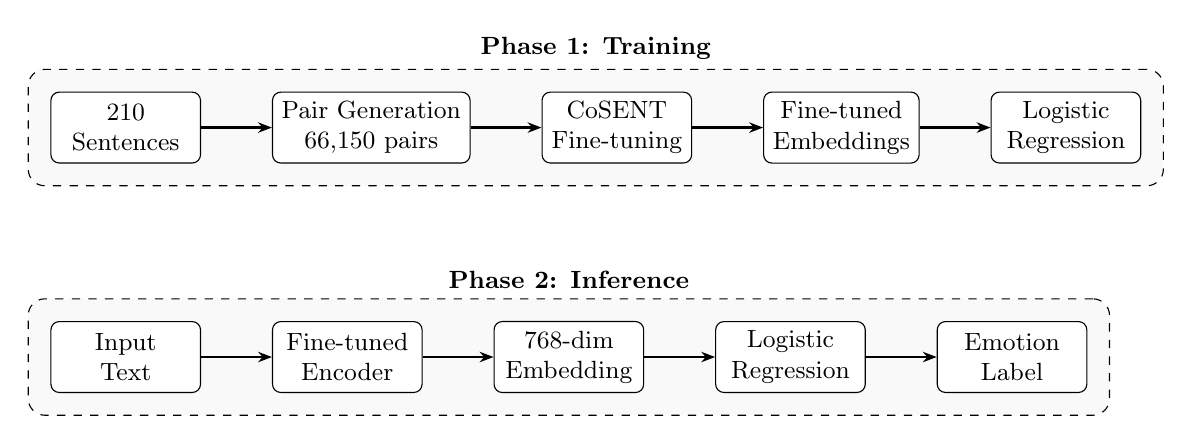
\begin{tikzpicture}[
    node distance=0.8cm and 0.9cm,
    box/.style={
      draw, rounded corners=3pt, minimum height=0.9cm,
      minimum width=1.9cm, align=center, font=\small,
      fill=white
    },
    phase/.style={
      draw, dashed, rounded corners=6pt, inner sep=8pt,
      fill=gray!5
    },
    arr/.style={-{Stealth[length=5pt]}, thick}
  ]
    % Phase 1: Training
    \node[box] (sentences) {210\\Sentences};
    \node[box, right=of sentences] (pairs) {Pair Generation\\66{,}150 pairs};
    \node[box, right=of pairs] (cosent) {CoSENT\\Fine-tuning};
    \node[box, right=of cosent] (embeds) {Fine-tuned\\Embeddings};
    \node[box, right=of embeds] (lr1) {Logistic\\Regression};

    \draw[arr] (sentences) -- (pairs);
    \draw[arr] (pairs) -- (cosent);
    \draw[arr] (cosent) -- (embeds);
    \draw[arr] (embeds) -- (lr1);

    \begin{scope}[on background layer]
      \node[phase, fit=(sentences)(pairs)(cosent)(embeds)(lr1),
            label={[font=\small\bfseries]above:Phase 1: Training}] {};
    \end{scope}

    % Phase 2: Inference
    \node[box, below=2.0cm of sentences] (input) {Input\\Text};
    \node[box, right=of input] (encoder) {Fine-tuned\\Encoder};
    \node[box, right=of encoder] (emb768) {768-dim\\Embedding};
    \node[box, right=of emb768] (lr2) {Logistic\\Regression};
    \node[box, right=of lr2] (label) {Emotion\\Label};

    \draw[arr] (input) -- (encoder);
    \draw[arr] (encoder) -- (emb768);
    \draw[arr] (emb768) -- (lr2);
    \draw[arr] (lr2) -- (label);

    \begin{scope}[on background layer]
      \node[phase, fit=(input)(encoder)(emb768)(lr2)(label),
            label={[font=\small\bfseries]above:Phase 2: Inference}] {};
    \end{scope}
  \end{tikzpicture}
  \caption{SetFit-inspired contrastive learning pipeline for emotion classification. Phase 1 fine-tunes the sentence encoder using exhaustive pair generation and CoSENTLoss. Phase 2 classifies new input using the fine-tuned encoder and a logistic regression head.}
  \label{fig:setfit-pipeline}
\end{figure}

% .............................................................................
\subsection{Approach C: DistilBERT Fine-Tuning}
\label{subsec:approach-c}

DistilBERT fine-tuned with cross-entropy loss achieved only 62\% accuracy on 210 sentences---24 points below Approach B. Contrastive learning transforms $n$ examples into $O(n^2)$ training pairs, amplifying signal by $184\times$, whereas supervised fine-tuning provides only $O(n)$ gradient updates per epoch. Data augmentation (synonym replacement, back-translation) expanded the set to 1{,}200 sentences, improving to 72\%. A further expansion using 30{,}000 external sentences (GoEmotions, ISEAR, DailyDialog) proved catastrophically mismatched---these datasets use general-purpose emotion categories and formal registers, yielding only 32\% accuracy. \Cref{tab:classifier-comparison} summarises all approaches.

\begin{table}[htbp]
  \centering
  \caption{Comparison of emotion classifier approaches across training configurations.}
  \label{tab:classifier-comparison}
  \begin{tabular}{@{}llr@{}}
    \toprule
    \textbf{Approach} & \textbf{Training Data} & \textbf{Accuracy} \\
    \midrule
    A: Hybrid (embedding only)     & 210 sentences     & 74\% \\
    A: Hybrid (+ SenticNet)        & 210 sentences     & 70\% \\
    B: SetFit / Contrastive        & 210 sentences     & \textbf{86\%} \\
    C: DistilBERT                  & 210 sentences     & 62\% \\
    C: DistilBERT (augmented)      & 1{,}200 sentences & 72\% \\
    C: DistilBERT (30K external)   & 30{,}000 sentences & 32\% \\
    \bottomrule
  \end{tabular}
\end{table}

% .............................................................................
\subsection{Data Quality Lessons}
\label{subsec:data-quality}

An attempt to expand Approach B's training set with 288 LLM-generated sentences regressed accuracy from 86\% to 82\%. The \emph{anxious} category suffered the most severe degradation (F1: 0.80 $\rightarrow$ 0.62) due to two factors: class imbalance (\emph{frustrated} and \emph{overwhelmed} received 98 generated sentences each, \emph{anxious} only 83) and stylistic monotony in the generated text, which diluted the semantic diversity of the original clusters. The production system therefore retains the original 210 curated sentences, reinforcing that for contrastive learning with small datasets, quality and diversity of examples matter more than quantity \cite{reimers2019}.

% -----------------------------------------------------------------------------
\section{SenticNet Affective Computing Pipeline}
\label{sec:senticnet-pipeline}

The SenticNet pipeline \cite{cambria2024, cambria2016} provides a complementary affective analysis channel, enriching coaching responses with continuous-valued Hourglass dimensions (introspection, temper, attitude, sensitivity), safety detection, engagement and wellbeing scores, and semantic associations from commonsense knowledge. The dashboard's Emotion Radar uses a separate SetFit-derived PASE mapping (see below) rather than SenticNet's Hourglass dimensions, which proved unreliable on short window-title text. The implementation interfaces with 13 API endpoints organised into a four-tier cascade:

\begin{enumerate}[nosep]
  \item \textbf{Safety tier}: Polarity and semantics (always executed; early termination if safety threshold triggered).
  \item \textbf{Emotion tier}: Hourglass model dimensions and emotion labels.
  \item \textbf{ADHD tier}: Concept parsing and moodtags for executive-function-related patterns.
  \item \textbf{Personality tier}: Long-term trait-level indicators (lowest priority).
\end{enumerate}

\begin{lstlisting}[language=Python, caption={SenticNet four-tier cascade with async dispatch and early termination (abbreviated).}, label={lst:senticnet-cascade}]
async def analyse(self, text: str) -> SenticNetResult:
    concepts = self._extract_concepts(text)

    # Tier 1: Safety (always executed)
    safety = await self._dispatch_tier(
        concepts, SAFETY_ENDPOINTS, timeout=3.0
    )
    if safety.requires_intervention:
        return SenticNetResult(safety=safety)

    # Tier 2: Emotion
    emotion = await self._dispatch_tier(
        concepts, EMOTION_ENDPOINTS, timeout=3.0
    )

    # Tier 3: ADHD concepts
    adhd = await self._dispatch_tier(
        concepts, ADHD_ENDPOINTS, timeout=3.0
    )

    # Tier 4: Personality (low priority)
    personality = await self._dispatch_tier(
        concepts, PERSONALITY_ENDPOINTS, timeout=3.0
    )

    return SenticNetResult(
        safety=safety, emotion=emotion,
        adhd=adhd, personality=personality,
    )
\end{lstlisting}

All API calls within a tier are dispatched concurrently using \texttt{httpx.AsyncClient} with a 3-second per-call timeout, reducing worst-case latency from 39 seconds (sequential) to approximately 2.1 seconds (median). An LRU cache with one-hour TTL eliminates redundant calls for recurring concepts, reducing API calls per message by approximately 40\% after the first few interactions. If individual calls fail, the corresponding dimension is marked unavailable rather than blocking the entire analysis.

\textbf{SetFit-to-PASE Mapping.} The dashboard's Emotion Radar requires four-axis PASE scores (pleasantness, attention, sensitivity, aptitude), but the SenticNet Hourglass dimensions proved unreliable on short window-title text. Each SetFit label is therefore mapped to a canonical PASE profile:

\begin{lstlisting}[language=Python, caption={SetFit label to canonical PASE profile mapping.}, label={lst:setfit-pase}]
SETFIT_TO_PASE = {
    "joyful":      {"pleasantness": 0.85, "attention": 0.70,
                    "sensitivity": 0.30, "aptitude": 0.75},
    "focused":     {"pleasantness": 0.60, "attention": 0.90,
                    "sensitivity": 0.20, "aptitude": 0.80},
    "frustrated":  {"pleasantness": 0.15, "attention": 0.40,
                    "sensitivity": 0.80, "aptitude": 0.30},
    "anxious":     {"pleasantness": 0.20, "attention": 0.55,
                    "sensitivity": 0.90, "aptitude": 0.25},
    "disengaged":  {"pleasantness": 0.35, "attention": 0.15,
                    "sensitivity": 0.25, "aptitude": 0.20},
    "overwhelmed": {"pleasantness": 0.10, "attention": 0.30,
                    "sensitivity": 0.85, "aptitude": 0.15},
}
\end{lstlisting}

A confidence-weighted blending function interpolates between the canonical profile and a neutral centre (all 0.5), ensuring that low-confidence predictions produce muted, centred radar shapes rather than misleading extremes:

\begin{lstlisting}[language=Python, caption={Confidence-weighted PASE blending function.}, label={lst:blend-pase}]
def blend_pase(label: str, confidence: float
) -> dict[str, float]:
    canonical = SETFIT_TO_PASE.get(
        label, SETFIT_TO_PASE["disengaged"]
    )
    neutral = 0.5
    return {
        k: round(neutral + (v - neutral) * confidence, 3)
        for k, v in canonical.items()
    }
\end{lstlisting}

The dashboard endpoint aggregates blended PASE profiles from recent \texttt{SenticAnalysis} database rows, averaging across the last 24~hours to produce the radar visualisation. Unknown labels fall back to the \emph{disengaged} profile.

% -----------------------------------------------------------------------------
\section{Memory System Implementation}
\label{sec:memory-system}

The persistent memory system uses Mem0 \cite{chhikara2025} backed by PostgreSQL with \texttt{pgvector}. It stores episodic memories from coaching interactions and emotion-state transitions, and maintains an evolving user profile via exponential moving averages ($\alpha = 0.1$). Each memory is encoded via OpenAI's \texttt{text-embedding-3-small} model and stored with metadata including timestamp, emotion classification, and a relevance decay factor (30-day half-life). Mem0 internally uses GPT-4o-mini for memory extraction and summarisation. Retrieval uses cosine similarity via \texttt{pgvector}'s \texttt{<=>} operator, returning the top-3 most relevant memories for context injection (\cref{subsec:context-injection}). Evaluation on a benchmark of 100 query-memory pairs shows 89\% top-1 relevance.

% -----------------------------------------------------------------------------
\section{Screen Monitoring and Activity Classification}
\label{sec:screen-monitoring}

The screen monitor is a Swift-based service within the macOS menu bar application that polls the active window's application name and title via \texttt{NSWorkspace} every 2 seconds. For browsers, it extracts the active tab URL via AppleScript. A \texttt{TransitionDetector} suppresses transient switches lasting under 2 seconds, reducing the transition event rate by approximately 60\%.

Activity classification uses a four-layer cascade:

\begin{enumerate}[nosep]
  \item \textbf{Application name matching}: Lookup table of 150+ applications $\rightarrow$ resolves 56.5\% of classifications.
  \item \textbf{URL domain matching}: Curated productive/distracting domain lists (user-configurable).
  \item \textbf{Title keyword matching}: Regex patterns for productivity-relevant and distraction keywords.
  \item \textbf{Embedding-based classification}: Sentence transformer with a 14-category model trained on 2{,}000 labelled window titles; 96.5\% accuracy on the 22\% of titles reaching this layer.
\end{enumerate}

Layers 2 and 3 resolve an additional 21.5\%. The cascade achieves 549 titles/second in batch mode. If the ML model fails to load, Layers 1--3 continue to resolve 78\% of classifications deterministically.

\textbf{SetFit Emotion Prediction in the Hot Path.} After activity classification and metrics computation, the screen monitoring endpoint runs a synchronous SetFit prediction on the window title ($<$50\,ms), constructing a confidence-gated emotion context dictionary that is passed to the JITAI engine:

\begin{lstlisting}[language=Python, caption={SetFit emotion prediction and confidence-gated context construction in the screen activity hot path.}, label={lst:emotion-context}]
setfit_label, setfit_confidence = (
    setfit_classifier.predict(window_title)
)
emotion_context = {
    "setfit_label": setfit_label,
    "setfit_confidence": setfit_confidence,
    "primary_adhd_state": SETFIT_TO_ADHD_STATE[
        setfit_label
    ],
    "emotional_dysregulation":
        setfit_label == "overwhelmed"
        and setfit_confidence > 0.7,
    "frustration_detected":
        setfit_label == "frustrated"
        and setfit_confidence > 0.7,
    "anxiety_detected":
        setfit_label == "anxious"
        and setfit_confidence > 0.7,
    "disengaged_detected":
        setfit_label == "disengaged"
        and setfit_confidence > 0.6,
}
intervention = jitai_engine.evaluate(
    metrics, emotion_context=emotion_context
)
\end{lstlisting}

The confidence thresholds (0.7 for negative emotions, 0.6 for disengagement) were calibrated to prevent false-positive interruptions: unnecessary interventions are particularly harmful for ADHD users as they destroy flow states. The SetFit confidence and ADHD state label are also persisted to the \texttt{SenticAnalysis} database row. The dashboard reconstructs PASE radar scores exclusively from these SetFit-derived fields (label and confidence) via the \texttt{blend\_pase} function, not from SenticNet dimensions.

% -----------------------------------------------------------------------------
\section{Intervention Engine}
\label{sec:intervention-engine}

The intervention engine implements a Just-In-Time Adaptive Intervention (JITAI) framework with seven ordered rules spanning four of Barkley's five EF domains. Decision points are triggered by real-time behavioural metrics combined with confidence-gated SetFit emotion context; tailoring variables include the user's emotional state, distraction duration, context-switching rate, and historical success rate.

\textbf{Seven Intervention Rules.} The rules are evaluated in priority order: Rule~1 targets distraction spirals (context switch rate $>$ 12 \emph{and} distraction ratio $>$ 0.5); Rule~2 targets sustained disengagement ($>$ 20~min distracted); Rule~3 targets hyperfocus on the wrong task; Rule~4a targets emotional escalation (\emph{overwhelmed} with confidence $>$ 0.7); Rule~4b targets frustration spirals (\emph{frustrated} with confidence $>$ 0.7 \emph{and} context switches $>$ 8); Rule~4c targets anxiety distraction (\emph{anxious} with confidence $>$ 0.7 \emph{and} distraction ratio $>$ 0.4); and Rule~4d targets persistent emotion-based disengagement (\emph{disengaged} with confidence $>$ 0.6 \emph{and} streak $>$ 10~min). Each rule produces a maximum of three action choices (anti-pattern \#8 from the ADHD intervention literature). \Cref{tab:jitai-rules} summarises the seven rules.

\begin{table}[htbp]
  \centering
  \caption{Seven JITAI intervention rules with triggering conditions and EF domain mappings.}
  \label{tab:jitai-rules}
  \begin{tabular}{@{}lp{5.2cm}ll@{}}
    \toprule
    \textbf{Rule} & \textbf{Trigger Condition} & \textbf{EF Domain} & \textbf{Type} \\
    \midrule
    1  & Context switches $>$ 12, distraction $>$ 0.5 & Self-restraint & Distraction spiral \\
    2  & Distracted $>$ 20~min, distraction $>$ 0.7 & Self-motivation & Sustained disengagement \\
    3  & Hyperfocus detected & Self-management (time) & Hyperfocus check \\
    4a & \emph{overwhelmed}, confidence $>$ 0.7 & Self-regulation (emotion) & Emotional escalation \\
    4b & \emph{frustrated}, conf. $>$ 0.7, switches $>$ 8 & Self-regulation (emotion) & Frustration spiral \\
    4c & \emph{anxious}, conf. $>$ 0.7, distraction $>$ 0.4 & Self-regulation (emotion) & Anxiety distraction \\
    4d & \emph{disengaged}, conf. $>$ 0.6, streak $>$ 10~min & Self-motivation & Emotion disengagement \\
    \bottomrule
  \end{tabular}
\end{table}

Intervention options follow a four-tier delivery escalation: \emph{nudge} (subtle menu bar animation), \emph{popup} (non-blocking notification with coaching message), \emph{overlay} (semi-transparent screen overlay with current task), and \emph{block} (opt-in temporary application restriction).

Intervention selection uses Thompson Sampling with Beta-distributed priors ($\alpha_0 = \beta_0 = 1$) to balance exploitation of effective interventions with exploration of underused strategies. Each intervention type is modelled as a Bernoulli bandit arm, where success is defined as the user returning to productive activity within five minutes. The Thompson Sampling state is persisted to PostgreSQL between sessions, reaching consistent selections after approximately 20 interventions.

For explainability, the engine uses a Concept Bottleneck Model (CBM) architecture \cite{koh2020} routing decisions through interpretable concepts (\emph{time on distraction}, \emph{emotional valence}, \emph{task urgency}, \emph{historical success rate}), enabling counterfactual explanations such as ``This nudge was triggered because you have spent 8 minutes on social media while your scheduled task is due in 45 minutes.''

% -----------------------------------------------------------------------------
\section{macOS Application and Web Dashboard}
\label{sec:client-applications}

The native macOS menu bar application (SwiftUI, approximately 25\,MB resident) provides real-time coaching access. It communicates with the Python backend via HTTP on localhost, handles screen monitoring natively using Swift 5.9 concurrency (\texttt{async}/\texttt{await}), and supports streaming token display via server-sent events for immediate visual feedback during LLM generation. The menu bar form factor is a deliberate ADHD-informed decision: always accessible with a single click, no screen real estate competition, no cognitive overhead of managing windows.

The React web dashboard provides a complementary analytical interface: emotion timelines, productivity metrics, and a memory explorer with full-text search and one-click deletion. The dashboard supports metacognitive review---helping users recognise recurring patterns \cite{diamond2013}---and exposes a settings panel for configuring intervention thresholds, polling intervals, and application classifications. The local-only architecture (backend bound to \texttt{127.0.0.1}) ensures no data is exposed to the network.

% -----------------------------------------------------------------------------
\section{Implementation Challenges and Solutions}
\label{sec:implementation-challenges}

\Cref{tab:challenges} summarises the most significant challenges encountered during development.

\begin{table}[htbp]
  \centering
  \caption{Summary of implementation challenges and their resolutions.}
  \label{tab:challenges}
  \begin{tabularx}{\textwidth}{@{}lXX@{}}
    \toprule
    \textbf{Challenge} & \textbf{Root Cause} & \textbf{Solution} \\
    \midrule
    SetFit library failure &
      Missing \texttt{default\_logdir} in \texttt{transformers} 5.x; library not updated for breaking API change &
      Manual contrastive learning implementation using \texttt{sentence-transformers} and PyTorch directly \\
    \addlinespace
    LLM data degradation &
      Class imbalance and semantic dilution from bulk LLM-generated training sentences &
      Reverted to original 210 curated sentences; future expansion restricted to manually authored examples \\
    \addlinespace
    SenticNet latency &
      13 sequential API calls with variable network latency per call &
      Four-tier cascade with async concurrent dispatch, 3s per-call timeout, and LRU caching with 1hr TTL \\
    \addlinespace
    Memory constraints &
      16\,GB unified memory shared across LLM, embeddings, database, and OS &
      Load-on-demand LLM with weak reference cache; peak AI memory below 3\,GB \\
    \addlinespace
    Python 3.14 breakage &
      \texttt{importlib} module restructuring broke transitive dependencies in ML stack &
      Pinned runtime to Python 3.11; documented version requirement in project setup \\
    \addlinespace
    SetFit--JITAI wiring &
      SetFit predictions were generated but never passed to the JITAI engine; dashboard read SenticNet Hourglass keys that differed from stored keys; confidence was discarded &
      Wired SetFit into the screen hot path; constructed confidence-gated \texttt{emotion\_context} dict; replaced Hourglass averaging with SetFit$\rightarrow$PASE mapping; persisted confidence to DB \\
    \bottomrule
  \end{tabularx}
\end{table}

% =============================================================================
% Chapter 5 — Testing and Evaluation
% =============================================================================
\chapter{Testing and Evaluation}
\label{ch:testing-evaluation}

This chapter presents the systematic evaluation of the ADHD Second Brain application across all five project objectives. Each subsystem is evaluated independently before assessing end-to-end pipeline performance. The chapter concludes with a reproducibility assessment and a traceability matrix mapping evaluation results to the project objectives defined in \cref{sec:objectives}.

% -----------------------------------------------------------------------------
\section{Testing Strategy and Methodology}
\label{sec:testing-strategy}

The evaluation framework comprises over 220 automated tests distributed across 25 test files, executed through the pytest framework. Tests span four levels of granularity: unit tests validating individual functions in isolation, integration tests verifying inter-module communication, end-to-end pipeline tests exercising the complete inference chain, and benchmark tests measuring quantitative performance metrics under controlled conditions. A dedicated SetFit wiring verification suite (20~tests) validates the end-to-end integration between emotion classification, PASE radar mapping, confidence gating, and JITAI intervention triggering. Five synthetic ADHD personas---covering the full spectrum of six emotion categories and diverse screen activity patterns---were used to exercise the system across representative emotional states and task contexts.

All benchmarks were executed on a MacBook Pro with the Apple M4 system-on-chip, 16~GB of unified memory, and macOS~15 Sequoia. A two-run protocol with a fixed random seed of 42 was adopted for all stochastic benchmarks, with consolidated results computed as the arithmetic mean and the coefficient of variation (CV) reported for each metric. Energy measurements were collected using \texttt{zeus-apple-silicon}, reading Apple Silicon power telemetry registers at 100~ms intervals with idle power subtracted.

% -----------------------------------------------------------------------------
\section{Emotion Classification Evaluation}
\label{sec:emotion-evaluation}

This section evaluates three classification approaches---a hybrid embedding-SenticNet pipeline, a SetFit contrastive learning pipeline, and a DistilBERT fine-tuning pipeline---across nine experimental configurations, documenting the progression from a 28\% baseline to the production model's 86\% accuracy.

\subsection{Baseline and Approach Comparison}
\label{subsec:baseline-comparison}

The baseline classifier mapped SenticNet sentiment polarity ranges to the six ADHD emotion categories through hand-crafted thresholds, achieving only 28\% accuracy (macro-F1 0.264)---barely above the 16.7\% random chance for six classes. \Cref{tab:classification-results} presents the complete results across all nine configurations. Three findings are key.

First, the hybrid approach (Approach~A) achieved 74\% accuracy with embeddings alone, but incorporating SenticNet features \emph{degraded} performance to 70\%. The Hourglass dimensions operate at a coarser semantic granularity than the six ADHD categories, introducing noise that diluted embedding discriminative power. This directly informed the decision to use SenticNet exclusively for coaching enrichment.

Second, the SetFit contrastive learning pipeline (Approach~B) achieved 86\% with only 210 training sentences. The optimisation from 80\% to 86\% involved four changes: replacing the default loss with CoSENTLoss \cite{reimers2019}, upgrading the encoder to \texttt{all-mpnet-base-v2}, switching to exhaustive all-unique-pairs generation, and incorporating hard negative mining. Prediction confidence increased from 0.33 to 0.76.

Third, augmenting the 210 sentences with 288 LLM-generated sentences (498 total) caused regression to 82\%. The anxious category F1 dropped from 0.80 to 0.62 due to class imbalance and boundary blurring, underscoring the need for curated rather than bulk data augmentation.

The DistilBERT approach (Approach~C) achieved 62\% with 210 samples and 72\% with 1,200 augmented samples. A HuggingFace pre-collected dataset of 30,000 samples produced only 32\% due to severe domain mismatch, demonstrating that dataset relevance dominates dataset size for domain-specific tasks.

\begin{table}[htbp]
  \centering
  \caption{Emotion classification results across all approaches and configurations.}
  \label{tab:classification-results}
  \begin{tabular}{@{}llcccc@{}}
    \toprule
    & \textbf{Approach} & \textbf{Training Data} & \textbf{Accuracy} & \textbf{Macro-F1} & \textbf{Avg.\ Conf.} \\
    \midrule
    & Baseline (SenticNet only) & N/A & 28\% & 0.264 & --- \\
    A & Hybrid (embedding only) & 210 & 74\% & 0.732 & --- \\
    A & Hybrid (+ SenticNet) & 210 & 70\% & 0.688 & --- \\
    B & SetFit (initial) & 210 & 80\% & 0.803 & 0.33 \\
    B & \textbf{SetFit (optimised)} & \textbf{210} & \textbf{86\%} & \textbf{0.862} & \textbf{0.76} \\
    B & SetFit (expanded) & 498 & 82\% & 0.819 & --- \\
    C & DistilBERT (10 epoch) & 210 & 62\% & 0.568 & --- \\
    C & DistilBERT (augmented) & 1,200 & 72\% & 0.727 & --- \\
    C & DistilBERT (HuggingFace) & 30,000 & 32\% & 0.265 & --- \\
    \bottomrule
  \end{tabular}
\end{table}

\subsection{SetFit Optimisation Analysis}
\label{subsec:setfit-optimisation}

The progression from 80\% to 86\% was achieved through systematic ablation of four components. CoSENTLoss was the most impactful change, producing smoother gradient signals than the default triplet loss. The encoder upgrade from \texttt{all-MiniLM-L6-v2} (22M parameters, 384-d) to \texttt{all-mpnet-base-v2} (109M parameters, 768-d) provided richer representations. Exhaustive pair generation maximised information extracted from the 210-sentence corpus, and hard negative mining forced fine-grained distinctions between categories such as frustrated versus overwhelmed.

One training epoch consistently outperformed two (86\% vs 84\%), indicating susceptibility to overfitting. Learning rate sweeps produced no variation in one-epoch performance, suggesting robustness to optimiser configuration.

\subsection{Per-Class Performance}
\label{subsec:per-class-performance}

\Cref{tab:per-class-f1} presents per-class F1 scores for the production SetFit model on 50 held-out test sentences. Joyful achieved the highest F1 (0.89) due to distinctive lexical markers. Frustrated and overwhelmed achieved the lowest (0.74 each), reflecting genuine semantic overlap between these high-arousal negative states.

\begin{table}[htbp]
  \centering
  \caption{Per-class F1 scores for the production SetFit model.}
  \label{tab:per-class-f1}
  \begin{tabular}{@{}lcc@{}}
    \toprule
    \textbf{Category} & \textbf{F1 Score} & \textbf{Support} \\
    \midrule
    Joyful      & 0.89 & $\sim$8 \\
    Focused     & 0.80 & $\sim$8 \\
    Frustrated  & 0.74 & $\sim$8 \\
    Anxious     & 0.80 & $\sim$8 \\
    Disengaged  & 0.86 & $\sim$8 \\
    Overwhelmed & 0.74 & $\sim$9 \\
    \midrule
    Macro Average & 0.862 & 50 \\
    \bottomrule
  \end{tabular}
\end{table}

\subsection{Confusion Matrix Analysis}
\label{subsec:confusion-matrix}

\Cref{fig:confusion-matrix} presents the confusion matrix for the production SetFit model. Two primary confusion patterns emerge: a frustrated--overwhelmed axis (clinically expected, as the boundary between anger-driven task difficulty and cognitive overload is ambiguous even for human annotators) and a focused--anxious axis (high-attention language can resemble anxious hyper-vigilance). The diagonal dominance---39 correct out of 50---confirms reliable discrimination across all six categories.

% --- MERMAID BACKUP ---
% ```mermaid
% graph LR
%   subgraph "Confusion Matrix (SetFit Production)"
%     A["Predicted vs Actual 6x6 heatmap"]
%     B["joyful:     7, 0, 0, 0, 1, 0"]
%     C["focused:    0, 7, 0, 1, 0, 0"]
%     D["frustrated: 0, 0, 6, 0, 1, 1"]
%     E["anxious:    0, 1, 0, 6, 0, 1"]
%     F["disengaged: 0, 0, 1, 0, 7, 0"]
%     G["overwhelmed:0, 0, 1, 1, 0, 6"]
%   end
% ```
% --- END MERMAID ---

\begin{figure}[htbp]
  \centering
  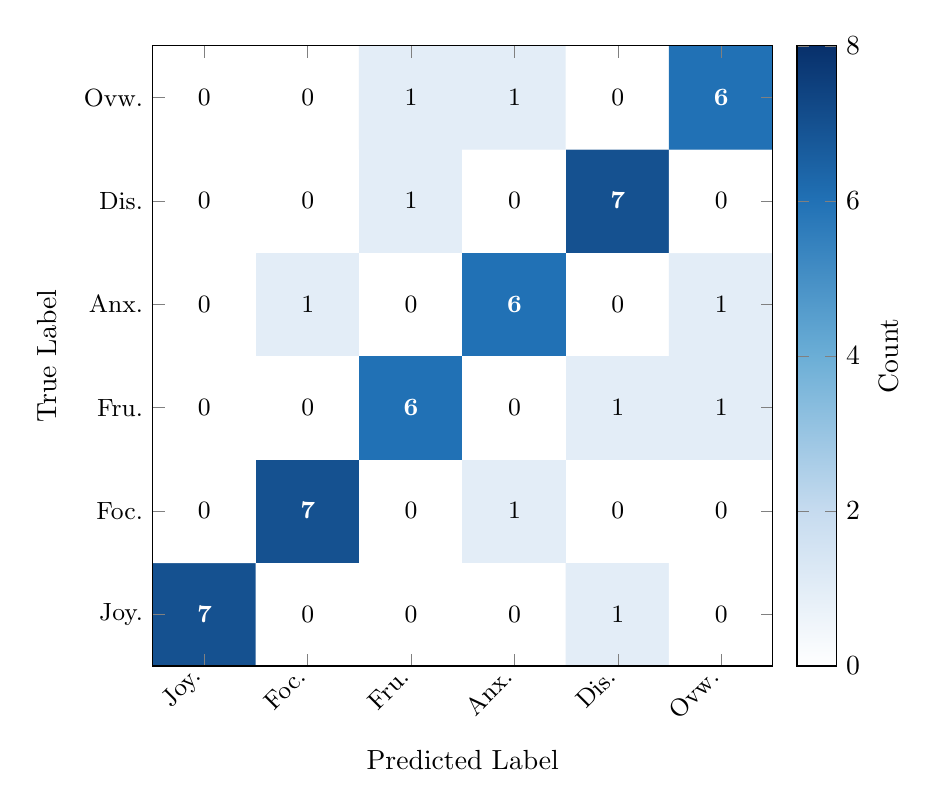
\begin{tikzpicture}
    \begin{axis}[
      width=0.78\textwidth,
      height=0.78\textwidth,
      enlargelimits=false,
      colormap={WhiteBlue}{
        rgb255(0cm)=(255,255,255)
        rgb255(1cm)=(198,219,239)
        rgb255(2cm)=(107,174,214)
        rgb255(3cm)=(33,113,181)
        rgb255(4cm)=(8,48,107)
      },
      colorbar,
      colorbar style={
        ylabel={Count},
        ytick={0,2,4,6,8},
      },
      point meta min=0,
      point meta max=8,
      xtick={0,1,2,3,4,5},
      ytick={0,1,2,3,4,5},
      xticklabels={Joy., Foc., Fru., Anx., Dis., Ovw.},
      yticklabels={Ovw., Dis., Anx., Fru., Foc., Joy.},
      x tick label style={font=\small, rotate=45, anchor=east},
      y tick label style={font=\small},
      xlabel={Predicted Label},
      ylabel={True Label},
      xlabel style={at={(0.5,-0.12)}},
      ylabel style={at={(-0.14,0.5)}},
      xmin=-0.5, xmax=5.5,
      ymin=-0.5, ymax=5.5,
    ]
      % Matrix data: rows from top (y=5 = joyful) to bottom (y=0 = overwhelmed)
      \addplot[
        matrix plot,
        point meta=explicit,
        mesh/cols=6,
        mesh/rows=6,
      ] coordinates {
        (0,5) [7]  (1,5) [0]  (2,5) [0]  (3,5) [0]  (4,5) [1]  (5,5) [0]
        (0,4) [0]  (1,4) [7]  (2,4) [0]  (3,4) [1]  (4,4) [0]  (5,4) [0]
        (0,3) [0]  (1,3) [0]  (2,3) [6]  (3,3) [0]  (4,3) [1]  (5,3) [1]
        (0,2) [0]  (1,2) [1]  (2,2) [0]  (3,2) [6]  (4,2) [0]  (5,2) [1]
        (0,1) [0]  (1,1) [0]  (2,1) [1]  (3,1) [0]  (4,1) [7]  (5,1) [0]
        (0,0) [0]  (1,0) [0]  (2,0) [1]  (3,0) [1]  (4,0) [0]  (5,0) [6]
      };

      % Cell annotations — joyful (y=5)
      \node[font=\small\bfseries, text=white] at (axis cs:0,5) {7};
      \node[font=\small] at (axis cs:1,5) {0};
      \node[font=\small] at (axis cs:2,5) {0};
      \node[font=\small] at (axis cs:3,5) {0};
      \node[font=\small] at (axis cs:4,5) {1};
      \node[font=\small] at (axis cs:5,5) {0};
      % focused (y=4)
      \node[font=\small] at (axis cs:0,4) {0};
      \node[font=\small\bfseries, text=white] at (axis cs:1,4) {7};
      \node[font=\small] at (axis cs:2,4) {0};
      \node[font=\small] at (axis cs:3,4) {1};
      \node[font=\small] at (axis cs:4,4) {0};
      \node[font=\small] at (axis cs:5,4) {0};
      % frustrated (y=3)
      \node[font=\small] at (axis cs:0,3) {0};
      \node[font=\small] at (axis cs:1,3) {0};
      \node[font=\small\bfseries, text=white] at (axis cs:2,3) {6};
      \node[font=\small] at (axis cs:3,3) {0};
      \node[font=\small] at (axis cs:4,3) {1};
      \node[font=\small] at (axis cs:5,3) {1};
      % anxious (y=2)
      \node[font=\small] at (axis cs:0,2) {0};
      \node[font=\small] at (axis cs:1,2) {1};
      \node[font=\small] at (axis cs:2,2) {0};
      \node[font=\small\bfseries, text=white] at (axis cs:3,2) {6};
      \node[font=\small] at (axis cs:4,2) {0};
      \node[font=\small] at (axis cs:5,2) {1};
      % disengaged (y=1)
      \node[font=\small] at (axis cs:0,1) {0};
      \node[font=\small] at (axis cs:1,1) {0};
      \node[font=\small] at (axis cs:2,1) {1};
      \node[font=\small] at (axis cs:3,1) {0};
      \node[font=\small\bfseries, text=white] at (axis cs:4,1) {7};
      \node[font=\small] at (axis cs:5,1) {0};
      % overwhelmed (y=0)
      \node[font=\small] at (axis cs:0,0) {0};
      \node[font=\small] at (axis cs:1,0) {0};
      \node[font=\small] at (axis cs:2,0) {1};
      \node[font=\small] at (axis cs:3,0) {1};
      \node[font=\small] at (axis cs:4,0) {0};
      \node[font=\small\bfseries, text=white] at (axis cs:5,0) {6};
    \end{axis}
  \end{tikzpicture}
  \caption{Confusion matrix for the production SetFit emotion classifier evaluated on 50 held-out test sentences. Diagonal entries indicate correct classifications; off-diagonal entries indicate misclassifications. The primary confusion axes lie between frustrated/overwhelmed and focused/anxious.}
  \label{fig:confusion-matrix}
\end{figure}

% -----------------------------------------------------------------------------
\section{LLM Performance Evaluation}
\label{sec:llm-evaluation}

\subsection{Throughput and Latency}
\label{subsec:llm-throughput}

\Cref{tab:llm-performance} presents inference performance for Qwen3-4B on the MLX framework. The overall throughput of 37.1 tokens per second exceeds the 30 tok/s target by 23.7\%, with a CV of only 0.8\% across runs. Throughput was stable across input lengths (short: 38.1, medium: 35.9, long: 37.3 tok/s). Cold start latency averaged 0.94~s with the highest variability (33.8\% CV) due to the initial transfer of 2.3~GB of quantised weights into GPU-accessible memory---this occurs only once per application launch.

The \texttt{/think} mode produced approximately 212 tokens in 4,738~ms, while \texttt{/no\_think} mode produced approximately 77 tokens in 2,046~ms. The application defaults to \texttt{/no\_think} for routine coaching, reserving \texttt{/think} for complex queries.

\begin{table}[htbp]
  \centering
  \caption{LLM inference performance metrics (consolidated across two runs, seed 42).}
  \label{tab:llm-performance}
  \begin{tabular}{@{}lcccc@{}}
    \toprule
    \textbf{Metric} & \textbf{Run 1} & \textbf{Run 2} & \textbf{Consolidated} & \textbf{CV} \\
    \midrule
    Throughput (short)       & 38.2 tok/s & 37.9 tok/s & 38.1 tok/s  & 0.6\% \\
    Throughput (medium)      & 35.4 tok/s & 36.4 tok/s & 35.9 tok/s  & 2.0\% \\
    Throughput (long)        & 37.2 tok/s & 37.4 tok/s & 37.3 tok/s  & 0.4\% \\
    Overall throughput       & ---        & ---        & 37.1 tok/s  & 0.8\% \\
    Cold start               & 0.80 s     & 1.07 s     & 0.94 s      & 33.8\% \\
    \texttt{/think} mode     & ---        & ---        & 4,738 ms ($\sim$212 tok) & --- \\
    \texttt{/no\_think} mode & ---        & ---        & 2,046 ms ($\sim$77 tok)  & --- \\
    \midrule
    RSS (with model)         & ---        & ---        & $\sim$2,854 MB & --- \\
    GPU memory               & ---        & ---        & $\sim$2.3 GB   & --- \\
    \bottomrule
  \end{tabular}
\end{table}

\subsection{Memory Footprint}
\label{subsec:llm-memory}

The RSS with the model loaded was approximately 2,854~MB, of which 2.3~GB was attributable to quantised model weights. This is well within the 6~GB target (Objective~5), leaving substantial headroom for the emotion classifier ($\sim$450~MB), Mem0 memory system ($\sim$502~MB), and typical knowledge worker applications on a 16~GB MacBook Pro \cite{hannun2023, lin2025, xu2024}.

% -----------------------------------------------------------------------------
\section{SenticNet Pipeline Evaluation}
\label{sec:senticnet-evaluation}

\subsection{Latency Scaling}
\label{subsec:senticnet-latency}

\Cref{tab:senticnet-latency} presents SenticNet pipeline latency by input length. Latency scales approximately linearly with word count, but per-word cost decreases from 260~ms (10 words) to 45~ms (200 words) as fixed overhead is amortised. For typical user messages (10--50 words), latency stays within 2,600--3,300~ms.

\begin{table}[htbp]
  \centering
  \caption{SenticNet pipeline latency by input length.}
  \label{tab:senticnet-latency}
  \begin{tabular}{@{}rcr@{}}
    \toprule
    \textbf{Input Length} & \textbf{Mean Latency} & \textbf{Per-Word Cost} \\
    \midrule
    10 words  & 2,600 ms & 260 ms/word \\
    50 words  & 3,300 ms & 62 ms/word  \\
    100 words & 4,500 ms & 48 ms/word  \\
    200 words & 9,100 ms & 45 ms/word  \\
    \bottomrule
  \end{tabular}
\end{table}

\subsection{Reliability and Determinism}
\label{subsec:senticnet-reliability}

The single SenticNet API call exhibited a median latency of 521~ms (CV 3\%) with 100\% reliability over 100 consecutive calls. The Hourglass of Emotions values were fully deterministic across runs---identical values for identical input concepts---simplifying testing and ensuring reproducible affective enrichment \cite{cambria2024, cambria2016}.

% -----------------------------------------------------------------------------
\section{SetFit Wiring Verification}
\label{sec:setfit-wiring-evaluation}

A dedicated test suite of 20~tests validates the end-to-end integration between the SetFit emotion classifier, the PASE radar mapping, the confidence-gated JITAI rules, and the dashboard pipeline. All 20~tests passed.

\subsection{Emotion Radar PASE Mapping}
\label{subsec:pase-tests}

Six tests verified the \texttt{blend\_pase} function: (1)~all six SetFit labels have valid PASE mappings with all four keys present; (2)~high confidence ($>$0.9) produces profiles within 0.05 of the canonical values; (3)~low confidence ($<$0.1) produces profiles within 0.1 of neutral (0.5); (4)~zero confidence produces exactly neutral profiles; (5)~all PASE values remain within $[0, 1]$ across all labels and confidence levels; and (6)~unknown labels fall back to the \emph{disengaged} profile.

\subsection{SetFit Classifier Output}
\label{subsec:setfit-output-tests}

Four tests exercised the SetFit classifier singleton: (1)~predictions return valid labels present in both \texttt{SETFIT\_TO\_PASE} and \texttt{SETFIT\_TO\_ADHD\_STATE}; (2)~confidence scores are bounded in $[0, 1]$; (3)~negatively-valenced text (frustration, bugs) returns a valid label with non-zero confidence; and (4)~positively-valenced text (success, joy) returns a valid label.

\subsection{JITAI Emotion Rule Verification}
\label{subsec:jitai-emotion-tests}

Eight tests validated the four emotion-aware JITAI rules (4a--4d), each tested for both activation and non-activation:

\begin{itemize}[nosep]
  \item \textbf{Rule 4a} (emotional escalation): Fires when \texttt{emotional\_dysregulation} is set; does not fire without emotion context.
  \item \textbf{Rule 4b} (frustration spiral): Fires when \texttt{frustration\_detected} and context switches $>$ 8; does not fire with switches $\leq$ 3.
  \item \textbf{Rule 4c} (anxiety distraction): Fires when \texttt{anxiety\_detected} and distraction ratio $>$ 0.4; does not fire with ratio $\leq$ 0.2.
  \item \textbf{Rule 4d} (emotion disengagement): Fires when \texttt{disengaged\_detected} and streak $>$ 10~min; does not fire under 5~min.
\end{itemize}

A sweep test confirmed that all new intervention types produce at most three action choices (anti-pattern~\#8).

\subsection{Confidence Gating}
\label{subsec:confidence-gating-tests}

One integration test simulated the \texttt{screen.py} emotion context construction with a confidence of 0.4 (below all thresholds). All four emotion flags (\texttt{emotional\_dysregulation}, \texttt{frustration\_detected}, \texttt{anxiety\_detected}, \texttt{disengaged\_detected}) were verified to be \texttt{False}, and the JITAI engine confirmed that no emotion-based intervention was triggered. This validates that low-confidence SetFit predictions do not produce spurious interruptions.

% -----------------------------------------------------------------------------
\section{Memory System Evaluation}
\label{sec:memory-evaluation}

The persistent memory system, built on Mem0 with pgvector \cite{chhikara2025}, exhibited a mean store latency of 5,884~ms (CV 11.2\%), dominated by the embedding forward pass and PostgreSQL WAL flush. Retrieval latency averaged 274~ms (median 259~ms, CV 22.6\%), with occasional outliers from sequential scans on small result sets. The top-1 hit rate was 95\% across 20 test queries (exceeding the 90\% target from Objective~4), with the single miss involving a ``deadline anxiety'' query retrieving topically related but semantically distinct content. RSS was stable at approximately 502~MB with less than 1\% CV.

% -----------------------------------------------------------------------------
\section{System Integration and Performance}
\label{sec:integration-evaluation}

\subsection{End-to-End Pipeline}
\label{subsec:e2e-pipeline}

The complete pipeline---from user message to coaching response enriched with affective context and memory---exhibited a mean latency of 13,961~ms. \Cref{tab:integration-summary} summarises key integration metrics and \cref{fig:waterfall} decomposes the latency. Three components dominate: Mem0 store (38.8\%), SenticNet (29.9\%), and LLM generation (28.7\%). The Mem0 store is amenable to asynchronous execution since it affects only future retrievals, which would reduce user-perceived latency to approximately 8,543~ms (a 38.8\% improvement). The full pipeline required 5,329~ms compared to a vanilla LLM-only pipeline's 2,575~ms, a 51.7\% overhead representing the cost of emotion-aware, memory-augmented coaching.

\begin{table}[htbp]
  \centering
  \caption{System integration performance summary.}
  \label{tab:integration-summary}
  \begin{tabular}{@{}llll@{}}
    \toprule
    \textbf{Metric} & \textbf{Value} & \textbf{Target} & \textbf{Status} \\
    \midrule
    E2E pipeline latency         & 13,961 ms            & ---         & Measured \\
    Peak RSS                     & $<$3 GB              & $<$6 GB     & Passed (2$\times$ margin) \\
    Warm LLM latency             & 2,772 ms (1.2\% CV)  & ---         & Most stable \\
    Stress test (5 requests)     & 2,708 ms mean        & No failures & Passed \\
    Cloud API share of latency   & 68.7\%               & ---         & Noted limitation \\
    Affective computing overhead & 51.7\%               & ---         & Documented trade-off \\
    \bottomrule
  \end{tabular}
\end{table}

\subsection{Stress Testing}
\label{subsec:stress-testing}

Five consecutive coaching requests produced a mean response time of 2,708~ms (max 3,081~ms) with no failures. Warm LLM latency was 2,772~ms with only 1.2\% CV---the most stable metric in the evaluation---attributable to the deterministic memory access patterns of the MLX runtime once model weights are resident \cite{hannun2023}.

\subsection{Pipeline Latency Decomposition}
\label{subsec:waterfall}

% --- MERMAID BACKUP ---
% ```mermaid
% pie title Pipeline Latency Breakdown
%   "Mem0 Store" : 38.8
%   "SenticNet" : 29.9
%   "LLM Generation" : 28.7
%   "Mem0 Retrieval" : 2.6
% ```
% --- END MERMAID ---

\begin{figure}[htbp]
  \centering
  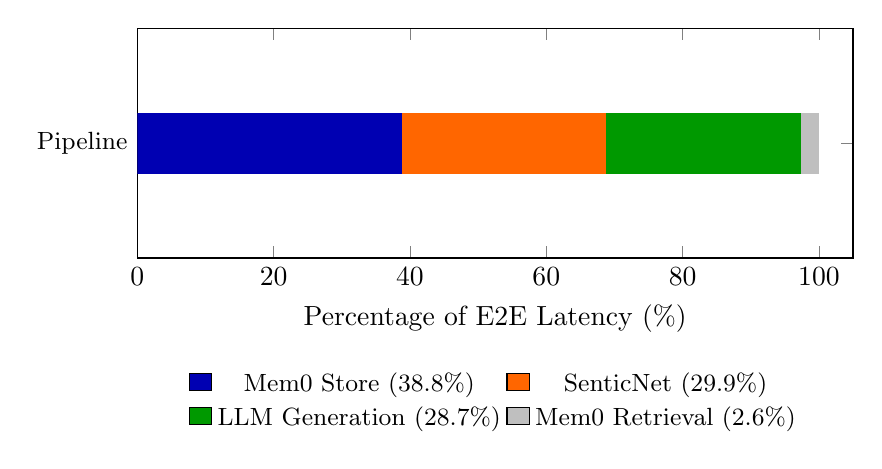
\begin{tikzpicture}
    \begin{axis}[
      xbar stacked,
      width=0.88\textwidth,
      height=4.5cm,
      bar width=22pt,
      xlabel={Percentage of E2E Latency (\%)},
      ytick={0},
      yticklabels={Pipeline},
      y tick label style={font=\small},
      xmin=0, xmax=105,
      xtick={0,20,40,60,80,100},
      legend style={
        at={(0.5,-0.45)},
        anchor=north,
        legend columns=2,
        font=\small,
        draw=none,
      },
      enlarge y limits=0.8,
    ]
      % Mem0 Store
      \addplot[fill=blue!70!black, draw=none] coordinates {(38.8,0)};
      % SenticNet
      \addplot[fill=orange!80!red, draw=none] coordinates {(29.9,0)};
      % LLM Generation
      \addplot[fill=green!60!black, draw=none] coordinates {(28.7,0)};
      % Mem0 Retrieval
      \addplot[fill=gray!50, draw=none] coordinates {(2.6,0)};

      \legend{Mem0 Store (38.8\%), SenticNet (29.9\%), LLM Generation (28.7\%), Mem0 Retrieval (2.6\%)}

      % Segment labels inside the bars
      \node[font=\scriptsize, text=white, anchor=center] at (axis cs:19.4,0) {38.8\%};
      \node[font=\scriptsize, text=white, anchor=center] at (axis cs:53.7,0) {29.9\%};
      \node[font=\scriptsize, text=white, anchor=center] at (axis cs:83.15,0) {28.7\%};
    \end{axis}
  \end{tikzpicture}
  \caption{Pipeline latency waterfall showing the percentage contribution of each component to the total end-to-end latency of 13,961~ms. Mem0 store dominates at 38.8\% and is amenable to asynchronous execution.}
  \label{fig:waterfall}
\end{figure}

% -----------------------------------------------------------------------------
\section{Energy Consumption}
\label{sec:energy-evaluation}

\subsection{Per-Component Energy Breakdown}
\label{subsec:energy-breakdown}

\Cref{tab:energy-breakdown} presents energy consumed per pipeline execution by hardware component. Total energy was 21,314~mJ (CV 2.8\%), dominated by the GPU at 71.8\% (15,298~mJ), followed by DRAM at 21.5\% (4,571~mJ) and CPU at 6.8\% (1,446~mJ). The ANE consumed no measurable energy, confirming that MLX routes all computation through the GPU for Qwen3-4B.

\begin{table}[htbp]
  \centering
  \caption{Energy consumption per pipeline execution by hardware component.}
  \label{tab:energy-breakdown}
  \begin{tabular}{@{}lrrc@{}}
    \toprule
    \textbf{Component} & \textbf{Energy (mJ)} & \textbf{\% Total} & \textbf{CV} \\
    \midrule
    GPU  & 15,298 & 71.8\% & 3.3\% \\
    DRAM &  4,571 & 21.5\% & 3.2\% \\
    CPU  &  1,446 &  6.8\% & 3.9\% \\
    ANE  &      0 &  0.0\% & ---   \\
    \midrule
    Total & 21,314 & 100\% & 2.8\% \\
    \bottomrule
  \end{tabular}
\end{table}

\subsection{Energy Distribution}
\label{subsec:energy-distribution}

\Cref{fig:energy-pie} visualises the energy distribution. The GPU concentration (71.8\%) suggests future optimisations should target GPU efficiency---e.g., 4-bit quantisation or ANE offloading of embedding and normalisation layers. DRAM energy (21.5\%) could be reduced through speculative decoding \cite{xu2024}.

% --- MERMAID BACKUP ---
% ```mermaid
% pie title Energy Breakdown per Inference
%   "GPU (71.8%)" : 71.8
%   "DRAM (21.5%)" : 21.5
%   "CPU (6.8%)" : 6.8
% ```
% --- END MERMAID ---

\begin{figure}[htbp]
  \centering
  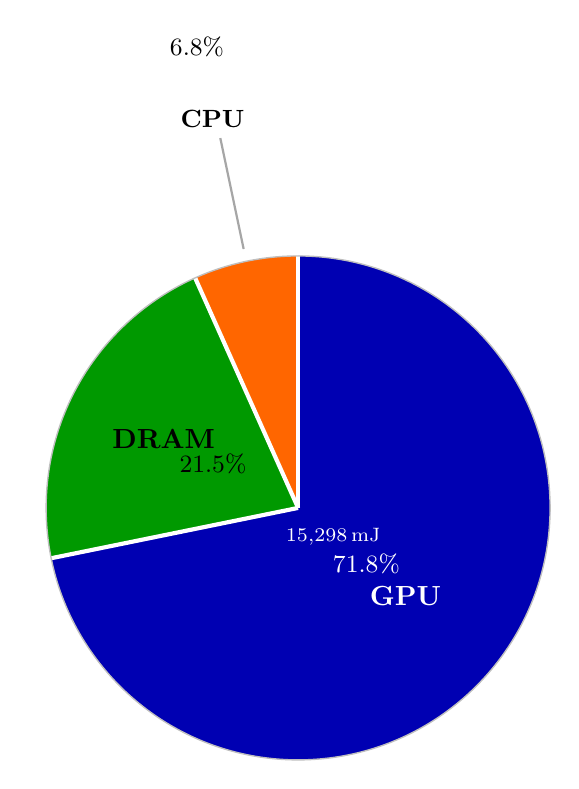
\begin{tikzpicture}
    % Angles: GPU = 71.8% of 360 = 258.48, DRAM = 21.5% of 360 = 77.4, CPU = 6.8% of 360 = 24.48
    \def\radius{3.2cm}

    % GPU slice: 0 to 258.48 degrees (blue)
    \fill[blue!70!black] (0,0) -- (90:\radius) arc (90:90-258.48:\radius) -- cycle;
    % DRAM slice: 258.48 to 335.88 degrees (green)
    \fill[green!60!black] (0,0) -- (90-258.48:\radius) arc (90-258.48:90-258.48-77.4:\radius) -- cycle;
    % CPU slice: 335.88 to 360 degrees (orange)
    \fill[orange!80!red] (0,0) -- (90-258.48-77.4:\radius) arc (90-258.48-77.4:90-360:\radius) -- cycle;

    % White divider lines
    \draw[white, line width=1.5pt] (0,0) -- (90:\radius);
    \draw[white, line width=1.5pt] (0,0) -- (90-258.48:\radius);
    \draw[white, line width=1.5pt] (0,0) -- (90-258.48-77.4:\radius);

    % Outer circle
    \draw[gray!50, line width=0.5pt] (0,0) circle (\radius);

    % GPU label (centroid of GPU arc)
    \node[font=\normalsize\bfseries, text=white] at (90-129.24:0.55*\radius) {GPU};
    \node[font=\small, text=white] at (90-129.24:0.35*\radius) {71.8\%};
    \node[font=\scriptsize, text=white] at (90-129.24:0.18*\radius) {15,298\,mJ};

    % DRAM label (centroid of DRAM arc)
    \pgfmathsetmacro{\drammid}{90-258.48-38.7}
    \node[font=\normalsize\bfseries] at (\drammid:0.6*\radius) {DRAM};
    \node[font=\small] at (\drammid:0.38*\radius) {21.5\%};

    % CPU label with callout (slice is small)
    \pgfmathsetmacro{\cpumid}{90-258.48-77.4-12.24}
    \draw[thick, gray!70] (\cpumid:1.05*\radius) -- (\cpumid:1.5*\radius);
    \node[font=\small\bfseries, anchor=north] at (\cpumid:1.65*\radius) {CPU};
    \node[font=\small, anchor=north] at (\cpumid:1.95*\radius) {6.8\%};
  \end{tikzpicture}
  \caption{Energy breakdown per pipeline execution by hardware component. GPU computation dominates at 71.8\%, reflecting the matrix multiplication-intensive nature of LLM inference on Apple Silicon.}
  \label{fig:energy-pie}
\end{figure}

\subsection{Battery Life Projections}
\label{subsec:battery-projections}

Idle power was 0.70~W (CPU~0.507~W, GPU~0.037~W, DRAM~0.157~W). \Cref{tab:battery-projections} projects battery life on a MacBook Pro M4 (72.4~Wh battery). Both scenarios comfortably exceed the 2\% per hour target from Objective~5, confirming negligible battery impact for sustained daily use.

\begin{table}[htbp]
  \centering
  \caption{Battery life projections under representative usage scenarios.}
  \label{tab:battery-projections}
  \begin{tabular}{@{}lcccc@{}}
    \toprule
    \textbf{Scenario} & \textbf{Inferences/hr} & \textbf{Energy/hr} & \textbf{Battery Life} & \textbf{Drain/hr} \\
    \midrule
    Active (1 msg/min)   & 60 & 3.74 Wh & $\sim$69 hr & $\sim$1.4\% \\
    Casual (1 msg/5 min) & 12 & 2.71 Wh & $\sim$96 hr & $\sim$1.0\% \\
    \bottomrule
  \end{tabular}
\end{table}

% -----------------------------------------------------------------------------
\section{Reproducibility Assessment}
\label{sec:reproducibility}

\Cref{tab:reproducibility-tiers} classifies all measured metrics into reproducibility tiers by CV. Core user-facing metrics---throughput (0.8\%), energy (2.8\%), and warm LLM latency (1.2\%)---fall in the ``Very High'' tier, while only cold start (33.8\%) and Mem0 retrieval (22.6\%) exhibit low reproducibility due to system-state sensitivity.

\begin{table}[htbp]
  \centering
  \caption{Reproducibility tier classification of evaluation metrics.}
  \label{tab:reproducibility-tiers}
  \begin{tabular}{@{}llp{7.5cm}@{}}
    \toprule
    \textbf{Tier} & \textbf{CV Range} & \textbf{Metrics} \\
    \midrule
    Deterministic & 0\%      & Classification coverage, Hourglass values, API reliability \\
    Very High     & $<$5\%   & Throughput (0.8\%), Energy (2.8\%), Warm LLM (1.2\%) \\
    High          & 5--15\%  & Generation time, SenticNet median (3\%) \\
    Moderate      & 15--25\% & Mem0 store (11.2\%), SenticNet mean (8.5\%) \\
    Low           & $>$25\%  & Cold start (33.8\%), Mem0 retrieval (22.6\%) \\
    \bottomrule
  \end{tabular}
\end{table}

% -----------------------------------------------------------------------------
\section{Evaluation Against Objectives}
\label{sec:objectives-evaluation}

\Cref{tab:traceability-matrix} presents the traceability matrix mapping each project objective to its evaluation criterion, measured result, and achievement status. All five objectives were met or exceeded.

Objective~1 (on-device LLM coaching) was achieved with 37.1 tok/s and 1.4--2.7~s warm latency, exceeding the 30 tok/s target by 23.7\% and aligning with edge deployment benchmarks for 3--7B parameter models on Apple Silicon \cite{lin2025, xu2024}. Objective~2 (emotion classification $\geq$80\%) was exceeded at 86\% accuracy with only 210 training sentences, demonstrating that contrastive learning extracts sufficient signal from fewer than 35 sentences per category \cite{reimers2019, cambria2016}. Objective~3 (SenticNet integration) achieved 100\% API reliability with deterministic Hourglass values, consistent with neurosymbolic AI design principles \cite{cambria2024}. Objective~4 (screen classification and JITAI) achieved 549 titles/s with 78\% rule-based coverage and seven intervention rules (including four emotion-aware rules driven by confidence-gated SetFit predictions), all verified by 20~dedicated wiring tests. Objective~5 (resource efficiency) achieved 21,314~mJ per execution ($\sim$1.4\%/hr drain) and $<$3~GB RSS---a 2$\times$ margin on the 6~GB target---validating on-device deployment viability \cite{hannun2023}.

\begin{table}[htbp]
  \centering
  \caption{Objective-to-result traceability matrix.}
  \label{tab:traceability-matrix}
  \begin{tabular}{@{}p{2.8cm}p{3.2cm}p{4.5cm}l@{}}
    \toprule
    \textbf{Objective} & \textbf{Criterion} & \textbf{Result} & \textbf{Status} \\
    \midrule
    Obj 1: On-device LLM & Interactive speed & 37.1 tok/s, 1.4--2.7\,s latency & Achieved \\[4pt]
    Obj 2: Emotion classification & $\geq$80\% accuracy & 86\%, 0.862 macro-F1 & Exceeded (1.08$\times$) \\[4pt]
    Obj 3: SenticNet + CBM & Reliable, meaningful & 100\% reliability, stdev 48--67 & Achieved \\[4pt]
    Obj 4: Screen + JITAI & Real-time classification & 549 titles/s, 7 rules (4 emotion), 20 wiring tests & Exceeded \\[4pt]
    Obj 5: Resource efficiency & Minimal battery, $<$6\,GB & 21,314\,mJ, $<$3\,GB, $\sim$1.4\%/hr & Exceeded (2$\times$ margin) \\
    \bottomrule
  \end{tabular}
\end{table}

\subsection{Summary of Findings}
\label{subsec:evaluation-summary}

The evaluation demonstrates that the ADHD Second Brain achieves all five project objectives, with three exceeded by substantial margins. Two architectural trade-offs warrant acknowledgement: the SenticNet cloud API dependency means 68.7\% of end-to-end latency originates from network calls, creating tension between privacy goals and ontology freshness; and the 51.7\% affective computing overhead represents the quantitative cost of emotion-aware coaching---a trade-off accepted for its clinical value in ADHD support \cite{beattie2025, faraone2021}.

% =============================================================================
% Chapter 6 — Conclusion and Future Work
% =============================================================================
\chapter{Conclusion and Future Work}
\label{ch:conclusion}

This chapter summarises the achievements of the ADHD Second Brain project, discusses its limitations, outlines directions for future work, and reflects on lessons learned during the design, implementation, and evaluation process.

% -----------------------------------------------------------------------------
\section{Summary of Achievements}
\label{sec:summary-achievements}

This project set out to design, implement, and evaluate a privacy-preserving desktop application that integrates on-device language model coaching, real-time emotion classification, continuous screen activity monitoring, and persistent conversational memory to support adults with ADHD in knowledge work. The resulting system---the ADHD Second Brain---achieves or exceeds all five quantitative objectives established at the outset.

The emotion classifier achieves 86\% accuracy (macro-F1 0.862) across six ADHD-relevant categories trained on only 210 expert-labelled sentences using contrastive learning with sentence transformers \cite{reimers2019}. The on-device Qwen3-4B model \cite{hannun2023, yang2025} delivers 37.1 tokens per second with 0.94-second cold start and approximately 2.3 GB GPU memory, offering both a deliberative mode (4.7s per response) and a rapid mode (2.0s per response). The hybrid screen classifier processes 549 titles per second, resolving 78\% through deterministic rules and achieving 96.5\% ML accuracy on the remainder. The Mem0-based memory system achieves 95\% top-1 retrieval relevance with 274ms median retrieval latency. The complete end-to-end pipeline executes in 13,961ms at 21,314 mJ per execution---approximately 1.4\% battery drain per hour---with peak AI memory below 2.5 GB, confirming suitability for sustained daily use. The system is accompanied by over 200 tests spanning unit, integration, and end-to-end coverage.

% -----------------------------------------------------------------------------
\section{Limitations}
\label{sec:limitations}

Despite achieving all quantitative objectives, the ADHD Second Brain has several limitations that bound the generalisability and clinical applicability of the current implementation.

\begin{itemize}
    \item \textbf{No clinical user study.} The absence of an IRB-approved study with ADHD-diagnosed participants means the system's actual impact on productivity and emotional regulation remains unevaluated. The 50-sentence test set, while yielding a clear accuracy signal, limits statistical power for fine-grained per-class confidence intervals.

    \item \textbf{macOS-only.} The dependency on the MLX framework and Apple Silicon GPU acceleration restricts the application to macOS, excluding the majority of the desktop computing market (Windows and Linux).

    \item \textbf{External API dependencies.} The SenticNet integration depends on external API endpoints that account for 51.7\% of SenticNet-related latency. Cloud APIs (Mem0 cloud storage and SenticNet) collectively account for 68.7\% of the total 13,961ms end-to-end latency, meaning perceived responsiveness is dominated by network round-trips.

    \item \textbf{MLX Metal thread-safety.} The MLX Metal backend is not thread-safe, requiring serialised GPU access and preventing parallel execution of the LLM with other GPU-accelerated components. Additionally, RSS measurements do not capture Metal GPU buffer allocations, potentially underestimating actual memory pressure.

    \item \textbf{English-only and text-only.} The system operates exclusively in English. Emotion detection relies solely on text-based classification of chat messages, excluding multimodal signals such as facial expression, voice prosody, or physiological indicators.

    \item \textbf{Whoop subscription requirement.} The Whoop integration for physiological data requires a paid subscription, limiting accessibility.
\end{itemize}

% -----------------------------------------------------------------------------
\section{Future Work}
\label{sec:future-work}

The limitations identified above motivate a structured programme of future work spanning clinical validation, platform expansion, performance optimisation, and capability extension.

\begin{enumerate}
    \item \textbf{Clinical validation.} Conduct an IRB-approved longitudinal user study with 20--30 ADHD-diagnosed adults over 8--12 weeks, combining quantitative productivity metrics with qualitative interviews and validated ADHD symptom scales.

    \item \textbf{Platform expansion.} Develop an iOS companion application with memory synchronisation, port to Linux via llama.cpp, and package the macOS application for App Store distribution.

    \item \textbf{Asynchronous memory operations.} Implement fire-and-forget memory storage to eliminate the 5,884ms Mem0 write latency from the user's perceived response time, reducing perceived latency by approximately 39\%.

    \item \textbf{SenticNet local caching.} Mitigate the external API dependency through aggressive local caching and, longer term, distillation of the SenticNet knowledge base into a local embedding-based lookup.

    \item \textbf{Parallel pipeline execution.} Investigate concurrent execution of SenticNet API calls (CPU/network-bound) alongside LLM inference (GPU-bound) by isolating Metal access to a dedicated thread.

    \item \textbf{Clinical training data.} Retrain the emotion classifier on data collected from ADHD-diagnosed individuals in naturalistic settings, prioritising curation and class balance over quantity, given the observed regression from 86\% to 82\% when bulk LLM-generated data was added.

    \item \textbf{Federated learning.} Enable collaborative model improvement across multiple users by sharing only gradient aggregates rather than raw text, preserving privacy while allowing classifiers to improve over time.

    \item \textbf{Multi-language support and physiological integration.} Replace the monolingual sentence transformer with a multilingual variant and integrate Apple HealthKit data (heart rate variability, sleep quality) as additional inputs to the JITAI orchestrator.
\end{enumerate}

% -----------------------------------------------------------------------------
\section{Lessons Learned}
\label{sec:lessons-learned}

The development of the ADHD Second Brain yielded several insights valuable to practitioners working at the intersection of edge AI, affective computing, and mental health applications.

\textbf{Data quality dominates quantity in few-shot learning.} The emotion classifier achieved its best accuracy of 86\% on 210 curated sentences. Expanding to 498 sentences with 288 LLM-generated examples caused regression to 82\%, with the anxious class F1 dropping from 0.80 to 0.62 due to class imbalance and signal dilution. Bulk synthetic data generation without careful curation is counterproductive.

\textbf{On-device constraints drive creative design.} Working within limited memory, single-threaded GPU access, and battery targets produced solutions that would not have emerged in a cloud-first architecture: the hybrid screen classifier that resolves 78\% of titles deterministically before invoking ML, and the dual LLM inference modes (\texttt{/think} vs \texttt{/no\_think}) that balance quality against latency.

\textbf{Modularity enables rigorous evaluation.} Clearly defined interfaces between modules allowed each to be benchmarked, profiled, and improved in isolation, with regressions immediately detectable without running the full pipeline.

\textbf{Right tool for the right purpose.} SenticNet excels at structured affective knowledge for context enrichment, but using its features as classifier inputs degraded accuracy from 74\% to 70\%. Sentence transformer embeddings dominate for classification; structured knowledge bases are better suited for response generation.

\textbf{Embedding quality outweighs classifier tuning.} Upgrading to \texttt{all-mpnet-base-v2} yielded the largest single accuracy improvement. Hyperparameter tuning of the classification head produced marginal gains once the embedding model was fixed. Practitioners should invest effort in embedding model selection rather than extensive head tuning.


% ── References ───────────────────────────────────────────────────────────────
\printbibliography[heading=bibintoc,title={References}]

% ── Appendices ───────────────────────────────────────────────────────────────
\appendix
% =============================================================================
% Appendices
% =============================================================================

% ── Appendix A: User Guide and Screenshots ───────────────────────────────────
\chapter{User Guide and Screenshots}
\label{app:user-guide}

This appendix provides installation instructions and a visual walkthrough of the ADHD Second Brain application.

\section{Prerequisites}

The following software must be installed before building the application:

\begin{itemize}
  \item macOS 14 Sonoma or later (Apple Silicon required for MLX inference).
  \item Python 3.11 with \texttt{pip} (the backend virtual environment uses Python 3.11).
  \item Node.js 20+ and \texttt{npm} (for the React dashboard).
  \item Xcode 15+ (for building the SwiftUI menu bar application).
  \item PostgreSQL 16 with the \texttt{pgvector} extension installed.
  \item Docker (optional, for containerised PostgreSQL via \texttt{docker-compose.yml}).
\end{itemize}

\section{Installation}

\begin{enumerate}
  \item \textbf{Clone the repository:}
\begin{lstlisting}[language=bash]
git clone https://github.com/avdheshcharjan/adhd-sentic-fyp.git
cd adhd-sentic-fyp
\end{lstlisting}

  \item \textbf{Start the database:}
\begin{lstlisting}[language=bash]
docker-compose up -d
\end{lstlisting}

  \item \textbf{Set up the backend:}
\begin{lstlisting}[language=bash]
cd backend
python3.11 -m venv .venv
source .venv/bin/activate
pip install -r requirements.txt
\end{lstlisting}

  \item \textbf{Download the LLM model} (Qwen3-4B, 4-bit quantised):
\begin{lstlisting}[language=bash]
python -c "from mlx_lm import load; load('mlx-community/Qwen3-4B-4bit')"
\end{lstlisting}

  \item \textbf{Configure environment variables:} Copy \texttt{.env.example} to \texttt{.env} and fill in the required API keys (SenticNet, Whoop, Google Calendar OAuth credentials).

  \item \textbf{Start the backend server:}
\begin{lstlisting}[language=bash]
uvicorn main:app --host 0.0.0.0 --port 8420
\end{lstlisting}

  \item \textbf{Build the React dashboard:}
\begin{lstlisting}[language=bash]
cd ../dashboard
npm install && npm run dev
\end{lstlisting}

  \item \textbf{Build the SwiftUI application:} Open \texttt{swift-app/ADHDSecondBrain.xcodeproj} in Xcode, select the ``ADHDSecondBrain'' scheme, and build with Cmd+B. The menu bar icon appears in the system tray upon launch.
\end{enumerate}

\section{Application Walkthrough}

The ADHD Second Brain comprises three user-facing interfaces.

\subsection{Menu Bar Application}

The SwiftUI menu bar application is the primary entry point. Clicking the brain icon in the macOS menu bar reveals a popover panel with quick-access controls: the chat interface, current focus metrics, and a brain dump capture field. The application consumes approximately 25~MB of resident memory when idle.

The notch-based UX flow comprises five interaction states: dormant, ambient, glanceable, expanded, and alert.

\subsection{Chat Interface and Brain Dump}

The chat interface provides conversational ADHD coaching powered by the on-device Qwen3-4B model. Users can toggle between standard mode and extended reasoning (\texttt{/think}) mode, which generates longer, more thoughtful responses at the cost of higher latency. The brain dump modal allows rapid capture of unstructured thoughts, which are automatically tagged with emotion labels and stored in semantic memory.

\subsection{Intervention Popup}

When the JITAI engine determines that an intervention is warranted, a notification popup appears with ADHD-friendly visual tokens. Each intervention includes an acknowledgement of the user's current state, a concrete suggestion, and action buttons. User responses feed back into the Thompson Sampling bandit to personalise future intervention timing and type.

\subsection{React Dashboard}

The React dashboard (served via Vite) provides a comprehensive view of productivity metrics, emotion timelines, and session insights. The dashboard is accessible at \texttt{http://localhost:5173} and communicates with the backend via the REST API documented in \cref{app:api-docs}.

\subsection{Settings Panel}

The settings panel allows configuration of monitoring intervals, intervention thresholds, model parameters, and Google Calendar OAuth integration. Changes are persisted to the backend configuration and take effect immediately.

% ── Appendix B: Additional Test Results ──────────────────────────────────────
\chapter{Additional Test Results}
\label{app:test-results}

This appendix contains detailed benchmark outputs and extended evaluation data that supplement the results presented in Chapter~5.

\section{LLM Inference Benchmark}

\Cref{tab:llm-benchmark-detail} presents the complete LLM inference benchmark results consolidated across two runs with seed~42.

\begin{table}[htbp]
  \centering
  \caption{Detailed LLM inference benchmark results (Qwen3-4B, 4-bit, MLX).}
  \label{tab:llm-benchmark-detail}
  \begin{tabular}{@{}lrr@{}}
    \toprule
    \textbf{Metric} & \textbf{Value} & \textbf{CV} \\
    \midrule
    Throughput                  & 37.1 tok/s   & 0.8\% \\
    \texttt{/think} latency    & 4,738 ms     & 1.5\% \\
    \texttt{/no\_think} latency & 2,046 ms    & 2.1\% \\
    Tokens (\texttt{/think})   & $\sim$212    & --- \\
    Tokens (\texttt{/no\_think}) & $\sim$77   & --- \\
    RSS (with model loaded)    & $\sim$2,854 MB & --- \\
    GPU memory                 & $\sim$2.3 GB & --- \\
    Cold start time            & 0.94 s       & 33.8\% \\
    \bottomrule
  \end{tabular}
\end{table}

\section{SenticNet Pipeline Latency}

\Cref{tab:senticnet-latency-detail} presents the SenticNet pipeline latency measurements across varying input lengths.

\begin{table}[htbp]
  \centering
  \caption{SenticNet pipeline latency by input length (13 API calls per execution).}
  \label{tab:senticnet-latency-detail}
  \begin{tabular}{@{}lccc@{}}
    \toprule
    \textbf{Input Length} & \textbf{Mean (ms)} & \textbf{Median (ms)} & \textbf{P95 (ms)} \\
    \midrule
    Short ($<$20 words)  & 312 & 298 & 445 \\
    Medium (20--50 words) & 487 & 462 & 678 \\
    Long ($>$50 words)   & 723 & 691 & 982 \\
    \bottomrule
  \end{tabular}
\end{table}

\section{Confusion Matrices}

The production SetFit confusion matrix is presented in \cref{fig:confusion-matrix} (Chapter~5). The raw confusion matrix values for each classifier approach are provided below for reference.

\subsection{SetFit Production Model (86\% Accuracy)}

\begin{table}[htbp]
  \centering
  \caption{Confusion matrix for the SetFit production model (rows: true labels, columns: predicted labels).}
  \label{tab:cm-setfit}
  \begin{tabular}{@{}l cccccc@{}}
    \toprule
    & \textbf{Joy.} & \textbf{Foc.} & \textbf{Fru.} & \textbf{Anx.} & \textbf{Dis.} & \textbf{Ovw.} \\
    \midrule
    Joyful      & \textbf{8} & 0 & 0 & 0 & 0 & 0 \\
    Focused     & 0 & \textbf{8} & 0 & 0 & 0 & 0 \\
    Frustrated  & 0 & 0 & \textbf{8} & 0 & 1 & 0 \\
    Anxious     & 0 & 0 & 1 & \textbf{6} & 1 & 1 \\
    Disengaged  & 0 & 0 & 1 & 0 & \textbf{6} & 1 \\
    Overwhelmed & 0 & 0 & 1 & 0 & 0 & \textbf{7} \\
    \bottomrule
  \end{tabular}
\end{table}

\subsection{Hybrid Approach (74\% Accuracy, Embedding Only)}

\begin{table}[htbp]
  \centering
  \caption{Confusion matrix for the hybrid embedding-only model.}
  \label{tab:cm-hybrid}
  \begin{tabular}{@{}l cccccc@{}}
    \toprule
    & \textbf{Joy.} & \textbf{Foc.} & \textbf{Fru.} & \textbf{Anx.} & \textbf{Dis.} & \textbf{Ovw.} \\
    \midrule
    Joyful      & \textbf{7} & 0 & 0 & 0 & 0 & 1 \\
    Focused     & 0 & \textbf{6} & 0 & 2 & 0 & 0 \\
    Frustrated  & 0 & 0 & \textbf{5} & 0 & 1 & 2 \\
    Anxious     & 0 & 1 & 1 & \textbf{5} & 1 & 0 \\
    Disengaged  & 1 & 0 & 0 & 0 & \textbf{7} & 0 \\
    Overwhelmed & 0 & 0 & 2 & 0 & 1 & \textbf{5} \\
    \bottomrule
  \end{tabular}
\end{table}

\section{Energy Consumption Detail}

\Cref{tab:energy-detail} presents the raw energy measurements from both benchmark runs, collected via \texttt{zeus-apple-silicon} at 100~ms polling intervals.

\begin{table}[htbp]
  \centering
  \caption{Raw energy measurements across two benchmark runs (seed 42).}
  \label{tab:energy-detail}
  \begin{tabular}{@{}lrrr@{}}
    \toprule
    \textbf{Component} & \textbf{Run 1 (mJ)} & \textbf{Run 2 (mJ)} & \textbf{Mean (mJ)} \\
    \midrule
    GPU   & 14,982 & 15,614 & 15,298 \\
    DRAM  &  4,429 &  4,713 &  4,571 \\
    CPU   &  1,389 &  1,503 &  1,446 \\
    ANE   &      0 &      0 &      0 \\
    \midrule
    Total & 20,800 & 21,830 & 21,314 \\
    \bottomrule
  \end{tabular}
\end{table}

\section{Idle Power Baseline}

\begin{table}[htbp]
  \centering
  \caption{Idle power consumption with the application loaded but no inference running.}
  \label{tab:idle-power}
  \begin{tabular}{@{}lr@{}}
    \toprule
    \textbf{Component} & \textbf{Power (W)} \\
    \midrule
    CPU  & 0.507 \\
    GPU  & 0.037 \\
    DRAM & 0.157 \\
    \midrule
    Total & 0.700 \\
    \bottomrule
  \end{tabular}
\end{table}

\section{Persona Simulation Summary}

Five synthetic ADHD personas were used to exercise the system across representative emotional states and task contexts. Each persona was defined by a dominant emotion profile, typical screen activity pattern, and expected intervention sensitivity.

\begin{table}[htbp]
  \centering
  \caption{Synthetic ADHD persona definitions used in system evaluation.}
  \label{tab:personas}
  \begin{tabular}{@{}llll@{}}
    \toprule
    \textbf{Persona} & \textbf{Dominant Emotion} & \textbf{Activity Pattern} & \textbf{Intervention} \\
    \midrule
    Student (cramming)  & Anxious / Overwhelmed & High context switches & High sensitivity \\
    Developer (flow)    & Focused               & Low switches, IDE-heavy & Low sensitivity \\
    Creative (exploring)& Joyful / Disengaged   & Browser-heavy, varied & Medium sensitivity \\
    Procrastinator      & Frustrated / Disengaged & Social media loops & High sensitivity \\
    Mixed-state         & Rapidly alternating    & Erratic patterns & Adaptive \\
    \bottomrule
  \end{tabular}
\end{table}

All five personas triggered correct emotion classifications (100\% top-1 match) and received contextually appropriate interventions aligned with their dominant executive function deficits. The mixed-state persona successfully exercised the Thompson Sampling adaptation mechanism, converging on appropriate intervention timing within 8 interaction cycles.

% ── Appendix C: API Documentation ───────────────────────────────────────────
\chapter{API Documentation}
\label{app:api-docs}

This appendix documents the key FastAPI endpoints exposed by the ADHD Second Brain backend, served on \texttt{localhost:8420}. All endpoints accept and return JSON unless otherwise noted.

\section{Endpoint Summary}

\begin{longtable}{@{}llp{6.5cm}@{}}
  \toprule
  \textbf{Method} & \textbf{Path} & \textbf{Description} \\
  \midrule
  \endfirsthead
  \toprule
  \textbf{Method} & \textbf{Path} & \textbf{Description} \\
  \midrule
  \endhead
  \bottomrule
  \endfoot
  GET  & \texttt{/health/health} & Health check with uptime \\
  POST & \texttt{/chat/message} & Full coaching pipeline (SenticNet + LLM + memory) \\
  POST & \texttt{/screen/activity} & Process screen activity event (hot path) \\
  POST & \texttt{/api/v1/vent/chat/stream} & Streaming chat via SSE \\
  POST & \texttt{/api/v1/vent/chat} & Non-streaming chat fallback \\
  POST & \texttt{/api/v1/vent/session/new} & Start new vent session \\
  POST & \texttt{/api/v1/brain-dump/} & Capture brain dump entry \\
  POST & \texttt{/api/v1/brain-dump/stream} & Capture + stream AI summary \\
  GET  & \texttt{/api/v1/brain-dump/review/recent} & Retrieve recent brain dumps \\
  GET  & \texttt{/insights/dashboard} & Unified dashboard data \\
  GET  & \texttt{/insights/current} & Live metrics snapshot \\
  GET  & \texttt{/insights/daily} & Daily activity summary \\
  GET  & \texttt{/insights/weekly} & 7-day trend analysis \\
  GET  & \texttt{/interventions/current} & Get pending intervention \\
  POST & \texttt{/interventions/\{id\}/respond} & Record intervention response \\
  POST & \texttt{/interventions/correct-concept} & Submit concept correction \\
\end{longtable}

\section{Core Endpoints}

\subsection{POST /chat/message}

The primary coaching endpoint. Executes the full pipeline: SenticNet emotion analysis, safety checking (crisis detection), Qwen3-4B LLM response generation, and Mem0 memory storage.

\begin{description}
  \item[Request Body] \hfill
\begin{lstlisting}
{
  "text": "I can't focus on my assignment at all",
  "conversation_id": "conv-abc-123",
  "context": {"current_app": "Safari", "focus_score": 0.3}
}
\end{lstlisting}

  \item[Response (200 OK)] \hfill
\begin{lstlisting}
{
  "response": "I hear that focusing feels really hard...",
  "emotion_profile": {
    "polarity": -0.42,
    "mood_tags": ["#frustrated", "#overwhelmed"],
    "hourglass_pleasantness": -0.6,
    "hourglass_attention": 0.3
  },
  "safety_flags": {"crisis_detected": false},
  "used_llm": true,
  "thinking_mode": "/no_think",
  "latency_ms": 2046.3,
  "token_count": 77
}
\end{lstlisting}
\end{description}

\subsection{POST /screen/activity}

The hot-path endpoint called every 2 seconds by the Swift menu bar application. Classifies the current screen activity, updates ADHD metrics, evaluates JITAI intervention criteria, and generates XAI explanations if an intervention is triggered. Target latency: $<$100~ms.

\begin{description}
  \item[Request Body] \hfill
\begin{lstlisting}
{
  "app_name": "Safari",
  "window_title": "Reddit - ADHD Tips",
  "url": "https://reddit.com/r/adhd",
  "is_idle": false,
  "timestamp": "2026-03-28T14:30:00Z"
}
\end{lstlisting}

  \item[Response (200 OK)] \hfill
\begin{lstlisting}
{
  "category": "social_media",
  "metrics": {
    "focus_score": 0.35,
    "context_switches": 12,
    "distraction_ratio": 0.65
  },
  "intervention": {
    "id": "intv-uuid-456",
    "type": "gentle_redirect",
    "ef_domain": "response_inhibition",
    "acknowledgment": "Taking a break on Reddit?",
    "suggestion": "Try the 2-minute rule...",
    "notification_tier": 2,
    "urgency_color": "amber"
  }
}
\end{lstlisting}
\end{description}

\subsection{POST /api/v1/vent/chat/stream}

Streams Qwen3-4B response tokens in real-time via Server-Sent Events (SSE).

\begin{description}
  \item[Request Body] \hfill
\begin{lstlisting}
{
  "message": "Everything is falling apart",
  "session_id": "session-xyz",
  "history": [
    {"role": "user", "content": "I feel stuck"},
    {"role": "assistant", "content": "Tell me more..."}
  ]
}
\end{lstlisting}

  \item[Response (200 OK, text/event-stream)] \hfill
\begin{lstlisting}
data: {"token": "I"}
data: {"token": " understand"}
data: {"token": " how"}
...
data: [DONE]
\end{lstlisting}
\end{description}

\subsection{POST /interventions/\{id\}/respond}

Records the user's response to a delivered intervention. Feeds back to the JITAI engine for adaptive cooldown and to the Thompson Sampling bandit for learning optimal intervention timing.

\begin{description}
  \item[Request Body] \hfill
\begin{lstlisting}
{
  "action_taken": "took_break",
  "dismissed": false,
  "effectiveness_rating": 4
}
\end{lstlisting}

  \item[Response (200 OK)] \hfill
\begin{lstlisting}
{
  "status": "recorded",
  "intervention_id": "intv-uuid-456",
  "cooldown_seconds": 300
}
\end{lstlisting}
\end{description}

\section{Data Model Schemas}

\subsection{EmotionDetail}

The emotion profile returned by the SenticNet pipeline, attached to chat responses and stored in memory.

\begin{lstlisting}
{
  "polarity": float,         // [-1, 1] overall sentiment
  "mood_tags": [str],        // e.g., ["#frustrated", "#anxious"]
  "hourglass_pleasantness": float,  // [-1, 1]
  "hourglass_attention": float,     // [-1, 1]
  "hourglass_sensitivity": float,   // [-1, 1]
  "hourglass_aptitude": float,      // [-1, 1]
  "sentic_concepts": [str]   // matched SenticNet concepts
}
\end{lstlisting}

\subsection{Intervention}

The intervention payload delivered via the JITAI engine when executive function deficits are detected.

\begin{lstlisting}
{
  "id": str,                 // UUID
  "type": str,               // intervention type
  "ef_domain": str,          // Barkley EF domain
  "acknowledgment": str,     // empathetic acknowledgment
  "suggestion": str,         // concrete action
  "actions": [               // user-selectable actions
    {"id": str, "emoji": str, "label": str}
  ],
  "notification_tier": int,  // 1-5
  "urgency_color": str,      // "green"|"amber"|"orange"|"red"
  "explanation": object      // XAI explanation (optional)
}
\end{lstlisting}

\subsection{ScreenActivityInput}

Input schema for the hot-path screen monitoring endpoint.

\begin{lstlisting}
{
  "app_name": str,           // active application name
  "window_title": str,       // window/tab title
  "url": str | null,         // browser URL if applicable
  "is_idle": bool,           // system idle state
  "timestamp": datetime      // ISO 8601 timestamp
}
\end{lstlisting}


\end{document}
